\documentclass[10pt]{beamer}
\usepackage[utf8x]{inputenc}
\usepackage{xspace}
\usepackage{tikz,pgfplots}
\usepackage{algorithm2e}
\usepackage{relsize}
\usepackage{comment}

\pgfplotsset{compat=1.9, width=1.0\textwidth, height=0.8\textheight}

\definecolor{darkred}{HTML}{A60000}
\definecolor{lightblue}{HTML}{366690}
\definecolor{darkgreen}{HTML}{009000}
\definecolor{lightbrown}{HTML}{AB6402}
\definecolor{yellow9}{HTML}{E1B640}

\mode<presentation>
{
  \setbeamercovered{transparent}
  \setbeamercolor{normal text}{fg=white,bg=gray}
  \setbeamercolor{alerted text}{fg=white}
  \setbeamercolor{example text}{fg=white}
  \setbeamercolor{background canvas}{bg=darkgray} 
  \setbeamercolor{structure}{fg=white}

  \setbeamercolor{block title}{bg=lightblue,fg=white}
  \setbeamercolor{block body}{bg=white,fg=darkgray}

  \setbeamercolor{block title example}{bg=lightblue,fg=white}
  \setbeamercolor{block body example}{bg=white,fg=darkgray}

  \setbeamercolor{palette primary}{use=normal text,fg=normal text.fg}
  \setbeamercolor{palette quaternary}{use=structure,fg=structure.fg}
  \setbeamercolor{palette secondary}{use=structure,fg=structure.fg}
  \setbeamercolor{palette tertiary}{use=normal text,fg=normal text.fg}

  \setbeamercolor{palette primary}{use=structure,fg=structure.fg}

  \setbeamercolor{math text}{}
  \setbeamercolor{math text inlined}{parent=math text}
  \setbeamercolor{math text displayed}{parent=math text}

  \setbeamercolor{enumerate item}{fg=lightgray}
  \setbeamercolor{itemize item}{fg=lightgray}
  \setbeamercolor{itemize subitem}{fg=lightgray}

  \setbeamercolor{normal text in math text}{}

  \setbeamercolor{local structure}{parent=structure}
  
  \setbeamercolor{titlelike}{parent=structure}

  \setbeamercolor{title}{parent=titlelike}
  \setbeamercolor{title in head/foot}{parent=palette quaternary}
  \setbeamercolor{title in sidebar}{parent=palette sidebar quaternary}

  \setbeamercolor{subtitle}{parent=title}

  \setbeamertemplate{navigation symbols}{}
}

\newcommand{\vectorbound}{\ensuremath{\kappa}}
\newcommand{\secretbound}{\ensuremath{\nu}}
\newcommand{\E}{\ensuremath{\textnormal{E}}}
\newcommand{\Var}{\ensuremath{\textnormal{Var}}}
\newcommand{\U}[1]{\ensuremath{\mathcal{U}(#1)\xspace}}
\newcommand{\abs}[1]{\ensuremath{|#1|}\xspace}
\newcommand{\dotp}[2]{\ensuremath{\left\langle {#1},{#2}\right\rangle}\xspace}

\newcommand{\shortvec}[1]{\tilde{\mathbf{#1}}\xspace}
\renewcommand{\vec}[1]{\mathbf{#1}\xspace}
\newcommand{\cemph}[1]{\color{yellow9}{\bf #1}\xspace}
\newcommand{\chig}{\ensuremath{\chi_{\alpha,q}}}
\newcommand{\Z}{\ensuremath{\mathbb{Z}}\xspace}
\newcommand{\Zq}{\ensuremath{\Z_q}\xspace}
\newcommand{\Zp}{\ensuremath{\mathbb{Z}_p}\xspace}
\newcommand{\Ldis}{L_{\mathbf{s},\chi}^{(n)}\xspace}
\newcommand{\sample}{\ensuremath{\leftarrow_{\$}}}
\renewcommand{\O}[1]{\ensuremath{{\mathcal{O}\left(#1\right)}}\xspace}
\newcommand{\round}[1]{\ensuremath{\left\lfloor{#1}\right\rceil}\xspace}
\newcommand{\Bdis}[1]{B_{\mathbf{s},\chi}(b,#1,p)\xspace}
\newcommand{\Bdissm}[1]{B_{small,\mathbf{s},\chi}(b,#1,p)\xspace}
\def\polyfactor{n\, \log_2^2 n}
\newcommand{\bigO}[1]{\ensuremath{\mathcal{O}\left(#1\right)}\xspace}


\newtheorem{assumption}{Assumption}

%%%%%%%%%%%%%%%%%%%%%%%%%%%%%%
% Presentation Title Content %
%%%%%%%%%%%%%%%%%%%%%%%%%%%%%%
\title{Solving LWE with BKW}
\author[Martin R.\ Albrecht]{Martin R.\ Albrecht\\{\small @martinralbrecht}\\{\small martinralbrecht@googlemail.com}}
\institute[Universities of Somewhere and Elsewhere] % (optional, but mostly needed)
{joint work with C.\ Cid, J.-C.\ Faugère, R.\ Fitzpatrick, and L.\ Perret}

\date{Lyon, 21.\ November 2013}

\AtBeginSection[] {
	\begin{frame}
		\frametitle{Contents}
		\tableofcontents[sectionstyle=show/shaded,subsectionstyle=show/shaded]
	\end{frame}
}

\AtBeginSubsection[] {
    \begin{frame}
        \frametitle{Contents}
        \tableofcontents[sectionstyle=show/shaded,subsectionstyle=show/shaded]
    \end{frame}
}

\begin{document}

\begin{frame}[plain] % frame of type 'plain' is an empty frame
  \titlepage
\end{frame}


%%%%%%%%%%%%%%%%%%%%%%%%%%%
% Table of Contents Slide %
%%%%%%%%%%%%%%%%%%%%%%%%%%%

\section{Introduction}

\begin{frame}
\frametitle{Learning with Errors}
\begin{definition}[Learning with Errors]
\begin{itemize}
\item Let $n\geq 1$, $m > n$, $q$ odd, $\chi$ be a probability distribution on $\Z_q$ and $\vec{s}$ be a secret vector in $\Z_q^n$.
\pause
\item Let $\vec{e} \sample \chi^m$, $\vec{A} \sample \U{\Z_q^{m \times n}}$. We denote by $\Ldis$ the distribution on $\Z_q^{m \times n} \times \Z_q^m$ produced as $(\vec{A}, \vec{A} \times \vec{s} + \vec{e})$.
\pause
\item Decision-LWE is the problem of deciding if\\$\vec{A},\vec{c} \sample \Ldis$ (i.e.\ $\vec{c} = \vec{A} \times \vec{s} + \vec{e}$ where $\vec{e}$ is ``small'') or\\ $\vec{A},\vec{c} \sample \U{\Z_q^{m\times n} \times \Z_q^{m}}$ (i.e.\ $\vec{c}$ is sampled uniformly random).
\end{itemize}
\end{definition}

\end{frame}

\pgfmathdeclarefunction{gauss}{2}{
  \pgfmathparse{1/(#2*sqrt(2*pi))*exp(-((x-#1)^2)/(2*#2^2))}
}
\begin{frame}
\frametitle{Small??}

\begin{columns}
\column{.4\textwidth}
\begin{itemize}
  \item<1-> We represent elements in $\Zq$ as integers in $[-\lfloor\frac{q}{2}\rfloor, \lfloor\frac{q}{2}\rfloor]$.
  \item<1-> By ``size'' we mean $\abs{x}$ for $x \in \Z_q$ in this representation.
  \item<2-> Typically, $\chi$ is a discrete Gaussian distribution over $\Z$ considered modulo $q$ with small standard deviation.
\end{itemize}

\column{.6\textwidth}
\hspace{-18em}\uncover<2->{\begin{tikzpicture}[scale=1]
  \begin{axis}[every axis plot post/.append style={mark=none,domain=-10:10,samples=50,smooth},
    axis x line*=bottom, % no box around the plot, only x and y axis
    axis y line*=left, % the * suppresses the arrow tips
    ] % extend the axes a bit to the right and top
   \addplot[color=lightblue,very thick] {gauss(0,3.0)};
  \end{axis}
\end{tikzpicture}}

\end{columns}
\end{frame}

\begin{frame}
\frametitle{Learning with Errors with Matrices}
 
We can generalise this slightly. Given $(\vec{A},\vec{C})$ with $\vec{C} \in \Zq^{m \times \ell}$, $\vec{A} \in \Zq^{m \times n}$, $\vec{S} \in \Zq^{n \times \ell}$ and $\vec{E} \in \Zq^{m \times \ell}$ do we have
\[
\left(
\begin{array}{ccc}
 \leftarrow & \ell & \rightarrow \\
 \\
 \\ 
 & \vec{C} & \\
 \\
 \\
 \\
\end{array} 
\right) = \left(
\begin{array}{ccc}
 \leftarrow & n & \rightarrow \\
 \\
 \\ 
 & \vec{A} & \\
 \\
 \\
 \\
\end{array} \right) \times \left( \begin{array}{ccc}
 \\ 
 & \vec{S} & \\
 \\
\end{array} \right) + \left(
\begin{array}{ccc}
 \leftarrow & \ell & \rightarrow \\
 \\
 \\ 
 & \vec{E} & \\
 \\
 \\
 \\
\end{array} 
\right)
\]
or $\vec{C} \sample \U{\Zq^{m \times \ell}}$.

\end{frame}


\begin{frame}
\frametitle{Applications}

\begin{itemize}
\item Public-Key Encryption, Digital Signature Schemes
\item Identity-based Encryption: encrypting to an identity (e-mail address \dots) instead of key
\item Fully-homomorphic encryption: computing with encrypted data
\item \dots
\end{itemize}
\end{frame}

\begin{frame}
\frametitle{Asymptotic Security}
Reduction of worst-case hard lattice problems such as Shortest Vector Problem (SVP) to average-case LWE.

\vspace{1em}

\begin{thebibliography}{foobar}
\bibitem{brakerski-langlois-peikert-regev-stehle:stoc13}
Z.\ Brakerski, A.\ Langlois, C.\ Peikert, O.\ Regev, and D.\ Stehl{\'e}.
\newblock Classical hardness of {L}earning with {E}rrors.
\newblock In {\em STOC '13}, pages 575--584, New York, 2013. ACM.
\end{thebibliography}

\pause

\vspace{1em}
 
\begin{block}{For cryptosystems we need the hardness of concrete instances:}
Given $m, n, q$ and $\chi$ how many operations does it take to solve Decision-LWE?
\end{block}



\end{frame}


\begin{frame}
\frametitle{Solving Strategies}

Given $\vec{A},\vec{c}$ with $\vec{c} = \vec{A} \times \vec{s} + \vec{e}$ or $\vec{c} \sample \U{\Zq^n}$

\vspace{1em}

\begin{itemize}

\item solve the Bounded-Distance Decoding (BDD) problem in the primal lattice: Find $\vec{s'}$ such that
\[
 \|\vec{y} - \vec{c}\| \textnormal{ is minimised, for } \vec{y} = \vec{A} \times \vec{s'}.
\]

\pause

\item Solve the Short-Integer-Solutions (SIS) problem in the scaled dual lattice. Find a short $\vec{y}$ such that
\[
 \vec{y} \times \vec{A} = 0 \textnormal{ and check if } \dotp{\vec{y}}{\vec{c}} = \vec{y}\times \left(\vec{A} \times \vec{s} + \vec{e}\right) = \dotp{\vec{y}}{\vec{e}} \textnormal{ is short.}
\]
\end{itemize}

\pause

\begin{block}{In this talk}
\begin{enumerate}
 \item we solve SIS 
 \item we use combinatorial techniques and
 \item we put no bound on $m$.
\end{enumerate}
\end{block}


\end{frame}


\section{Warm-Up: Deciding Consistency in Noise Free Systems}

\begin{frame}[allowframebreaks,fragile]
\frametitle{Gaussian elimination}
Asume there is no error, we hence want to decide whether there is a solution $\vec{s}$ such that $\vec{C} = \vec{A}\times \vec{S}$. We may apply Gaussian elimination to the matrix:
\[
\vec{[A\mid C]} = \left(\begin{array}{cccc|ccc}
\vec{a}_{11} & \vec{a}_{12} &  \dots & \vec{a}_{1n} & \vec{c}_{11} & \dots  & \vec{c}_{1\ell}\\
\vec{a}_{21} & \vec{a}_{22} &  \dots & \vec{a}_{2n} & \vec{c}_{21} & \dots  & \vec{c}_{2\ell}\\
\vdots       & \vdots       & \ddots & \vdots       & \vdots       & \ddots & \vdots\\
\vec{a}_{m1} & \vec{a}_{m2} & \dots  & \vec{a}_{mn} & c_{m1}       & \dots  & c_{m\ell}\\
\end{array}\right)
\]
to recover
\[
\vec{[\tilde A\mid \tilde C]} = \left(\begin{array}{cccc|ccc}
\vec{a}_{11} &      \vec{a}_{12} &  \dots & \vec{a}_{1n}      &      \vec{c}_{11} &  \dots &      \vec{c}_{1\ell}\\
           0 & \shortvec{a}_{22} &  \dots & \shortvec{a}_{2n} & \shortvec{c}_{21} &  \dots & \shortvec{c}_{2\ell}\\
      \vdots & \vdots            & \ddots & \vdots            & \vdots            & \ddots & \vdots \\
           0 & 0                 &  \dots & \shortvec{a}_{rn} & \shortvec{c}_{r1} &  \dots & \shortvec{c}_{r\ell}\\
      \vdots & \vdots            & \ddots & \vdots            & \vdots            & \ddots & \vdots \\
           0 & 0                 &  \dots & 0                 & \shortvec{c}_{m1} &  \dots & \shortvec{c}_{m\ell}\\
\end{array}\right)
\]

If and only if $\shortvec{c}_{r+1,1},\dots,\shortvec{c}_{m,\ell}$ are all zero, the system is consistent.

\framebreak

\vspace{-1.3em}
\begin{center}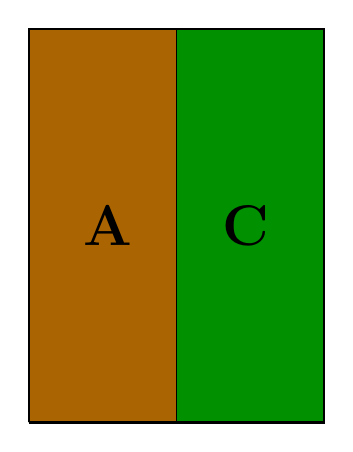
\begin{tikzpicture}[scale=0.25]
\draw[fill=darkgreen] (0,0) -- (0,20) -- (15,20) -- (15, 0) -- (0,0);
\draw[fill=lightbrown] (0,0) --(0,20) -- (7.5,20) -- (7.5,0) -- (0,0);
\node at (4, 10) {\huge $\vec{A}$};
\node at (11, 10) {\huge $\vec{C}$};
\draw[thick] (0,0) -- (0,20) -- (15,20) -- (15, 0) -- (0,0);
\end{tikzpicture}\end{center}

\framebreak

\begin{center}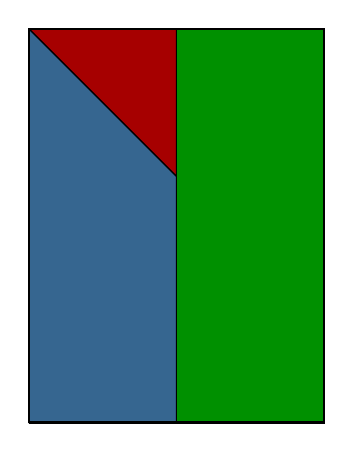
\begin{tikzpicture}[scale=0.25]
\draw[fill=darkgreen] (0,0) -- (0,20) -- ( 15,20) -- (15, 0) -- (0,0);
\draw[fill=white] (0,0) -- (0,20) -- (7.5,20) -- (7.5,0) -- (0,0);
\draw[fill=darkred] (0,20) -- (7.5,12.5) -- (7.5,20) -- (0,20);
\draw[fill=lightblue] (0,20) -- (7.5,12.5) -- (7.5,0) -- (0,0) -- (0,20);
\draw[thick] (0,0) -- (0,20) -- (15,20) -- (15, 0) -- (0,0);
\end{tikzpicture}\end{center}

\framebreak

\begin{center}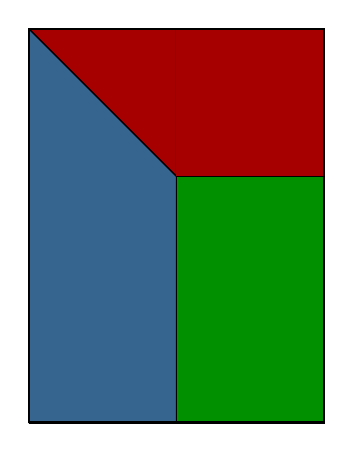
\begin{tikzpicture}[scale=0.25]
\draw[fill=darkgreen] (0,0) -- (0,20) -- ( 15,20) -- (15, 0) -- (0,0);
\draw[fill=white] (0,0) -- (0,20) -- (7.5,20) -- (7.5,0) -- (0,0);
\draw[fill=darkred] (0,20) -- (7.5,12.5) -- (7.5,20) -- (0,20);
\draw[fill=lightblue] (0,20) -- (7.5,12.5) -- (7.5,0) -- (0,0) -- (0,20);
\draw[fill=darkred] (7.5,20) -- (15,20) -- (15,12.5) -- (7.5,12.5);
\draw[thick] (0,0) -- (0,20) -- (15,20) -- (15, 0) -- (0,0);
\end{tikzpicture}\end{center}


\framebreak
\begin{center}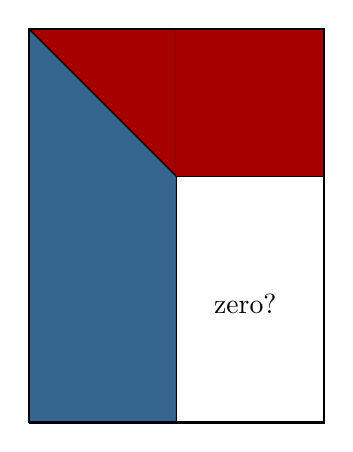
\begin{tikzpicture}[scale=0.25]
\draw[fill=white] (0,0) -- (0,20) -- ( 15,20) -- (15, 0) -- (0,0);
\draw[fill=darkred] (0,20) -- (7.5,12.5) -- (7.5,20) -- (0,20);
\draw[fill=lightblue] (0,20) -- (7.5,12.5) -- (7.5,0) -- (0,0) -- (0,20);
\draw[fill=darkred] (7.5,20) -- (15,20) -- (15,12.5) -- (7.5,12.5);
\node[black] at (11,6) {zero?};
\draw[thick] (0,0) -- (0,20) -- (15,20) -- (15, 0) -- (0,0);
\end{tikzpicture}\end{center}

\end{frame}




\section{Solving Decision-LWE}

\begin{frame}[allowframebreaks,fragile]
\frametitle{BKW Algorithm}

The BKW algorithm was first proposed for the Learning Parity with Noise (LPN) problem which can be viewed as a special case of LWE over $\Z_{2}$.

\vspace{1em}

\begin{thebibliography}{foobar}
\bibitem{DBLP:journals/jacm/BlumKW03}
Avrim Blum, Adam Kalai, and Hal Wasserman.
\newblock Noise-tolerant learning, the parity problem, and the statistical query model.
\newblock {\em J. ACM}, 50(4):506--519, 2003.
\end{thebibliography}

\framebreak

Goal in noise-free case:\phantom{$\Z_q$}

\begin{center}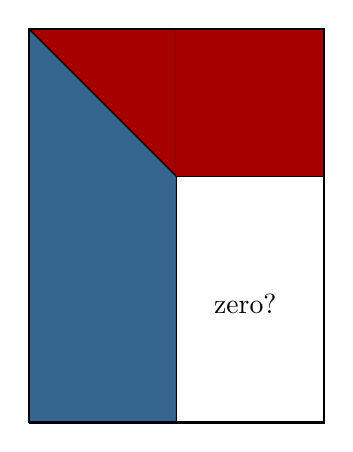
\begin{tikzpicture}[scale=0.25]
\draw[fill=white] (0,0) -- (0,20) -- ( 15,20) -- (15, 0) -- (0,0);
\draw[fill=darkred] (0,20) -- (7.5,12.5) -- (7.5,20) -- (0,20);
\draw[fill=lightblue] (0,20) -- (7.5,12.5) -- (7.5,0) -- (0,0) -- (0,20);
\draw[fill=darkred] (7.5,20) -- (15,20) -- (15,12.5) -- (7.5,12.5);
\node[black] at (11,6) {zero?};
\draw[thick] (0,0) -- (0,20) -- (15,20) -- (15, 0) -- (0,0);
\end{tikzpicture}\end{center}

\framebreak

Goal over $\Z_2$ (LPN):\phantom{$\Z_q$}

\begin{center}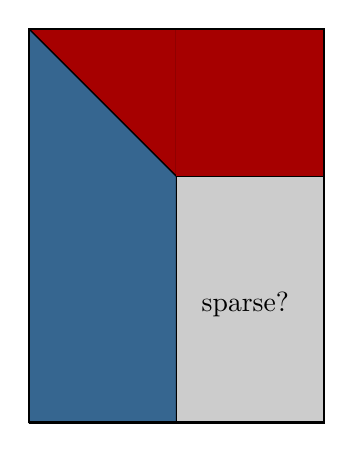
\begin{tikzpicture}[scale=0.25]
\draw[fill=black!20!white] (0,0) -- (0,20) -- ( 15,20) -- (15, 0) -- (0,0);
\draw[fill=white] (0,0) -- (0,20) -- (7.5,20) -- (7.5,0) -- (0,0);
\draw[fill=darkred] (0,20) -- (7.5,12.5) -- (7.5,20) -- (0,20);
\draw[fill=lightblue] (0,20) -- (7.5,12.5) -- (7.5,0) -- (0,0) -- (0,20);
\draw[fill=darkred] (7.5,20) -- (15,20) -- (15,12.5) -- (7.5,12.5);
\node[black] at (11,6) {sparse?};
\draw[thick] (0,0) -- (0,20) -- (15,20) -- (15, 0) -- (0,0);
\end{tikzpicture}\end{center}

\framebreak

Goal over $\Z_q$ (LWE):

\begin{center}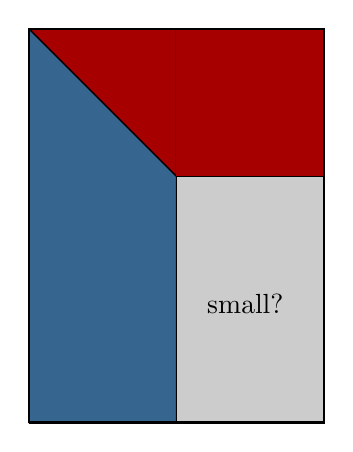
\begin{tikzpicture}[scale=0.25]
\draw[fill=black!20!white] (0,0) -- (0,20) -- ( 15,20) -- (15, 0) -- (0,0);
\draw[fill=white] (0,0) -- (0,20) -- (7.5,20) -- (7.5,0) -- (0,0);
\draw[fill=darkred] (0,20) -- (7.5,12.5) -- (7.5,20) -- (0,20);
\draw[fill=lightblue] (0,20) -- (7.5,12.5) -- (7.5,0) -- (0,0) -- (0,20);
\draw[fill=darkred] (7.5,20) -- (15,20) -- (15,12.5) -- (7.5,12.5);
\node[black] at (11,6) {small?};
\draw[thick] (0,0) -- (0,20) -- (15,20) -- (15, 0) -- (0,0);
\end{tikzpicture}\end{center}

\framebreak


We revisit Gaussian elimination:
\begin{eqnarray*}
& & \left(
\begin{array}{c|c|ccc|l}
\bold{a}_{11} & \bold{a}_{12} & \bold{a}_{13} & \cdots & \bold{a}_{1n} & c_1\\
\bold{a}_{21} & \bold{a}_{22} & \bold{a}_{23} & \cdots & \bold{a}_{2n} & c_2\\
\vdots & \vdots & \ddots & \vdots & \vdots\\
\bold{a}_{m1} & \bold{a}_{m2} & \bold{a}_{m3} & \cdots & \bold{a}_{mn} & c_{m}
\end{array}
\right)
\end{eqnarray*}

\begin{eqnarray*}
& \overset{?}{=} & \left(
\begin{array}{c|c|ccc|l}
\bold{a}_{11} & \bold{a}_{12} & \bold{a}_{13} & \cdots & \bold{a}_{1n} & \dotp{\vec{a}_1}{\vec{s}} + \vec{e}_1\\
\bold{a}_{21} & \bold{a}_{22} & \bold{a}_{23} & \cdots & \bold{a}_{2n} & \dotp{\vec{a}_2}{\vec{s}} + \vec{e}_2\\
\vdots & \vdots & \ddots & \vdots & \vdots\\
\bold{a}_{m1} & \bold{a}_{m2} & \bold{a}_{m3} & \cdots & \bold{a}_{mn} & \dotp{\vec{a}_m}{\vec{s}} + \vec{e}_m
\end{array}
\right)
\end{eqnarray*}

\framebreak

\begin{eqnarray*}
& \Rightarrow  & \left(
\begin{array}{c|c|ccc|l}
\bold{a}_{11} & \bold{a}_{12} & \bold{a}_{13} & \cdots & \bold{a}_{1n} & \dotp{\vec{a}_1}{\vec{s}} + \vec{e}_1\\
0 & \tilde{\bold{a}}_{22} & \tilde{\bold{a}}_{23} & \cdots & \tilde{\bold{a}}_{2n} & \dotp{\shortvec{a}_2}{\vec{s}} + \vec{e}_2 - \cemph{\frac{\bold{a}_{21}}{\bold{a}_{11}}\vec{e}_1}\\
\vdots & \vdots & \ddots & \vdots & \vdots\\
0 & \tilde{\bold{a}}_{m2} & \tilde{\bold{a}}_{m3} & \cdots & \tilde{\bold{a}}_{mn} & \dotp{\shortvec{a}_m}{\vec{s}} + \vec{e}_m - \cemph{\frac{\bold{a}_{m1}}{\bold{a}_{11}}\vec{e}_1}
\end{array}
\right)\phantom{\Longrightarrow}
\end{eqnarray*}

\begin{itemize}
 \item $\frac{\bold{a}_{i1}}{\bold{a}_{11}}$ is essentially a random element in $\Z_q$, hence $\tilde c_i \sample \U{\Z_q}$.
 \item Even if $\frac{\bold{a}_{i1}}{\bold{a}_{11}}$ is 1 the variance of the noise doubles at every level because of the addition.  
\end{itemize}

\framebreak

\begin{block}{The Problem and its Solution}
\begin{itemize}
 \item \textbf{Problem:} 
 \begin{itemize}
  \item \textbf{additions} increase density
  \item \textbf{multiplications} increase size
 \end{itemize}
 $\Rightarrow$ noise of $\shortvec{c}_{ij}$ values increases rapidly
 \item \textbf{Strategy:} exploit that we have many rows: $m \gg n$.
\end{itemize}
\end{block} 


\framebreak

Condition over $\Z_2$ (LPN):\phantom{$\Z_q$}

\begin{center}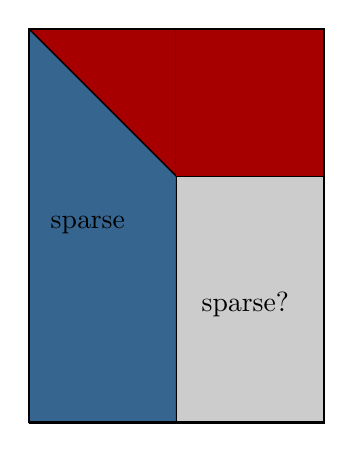
\begin{tikzpicture}[scale=0.25]
\draw[fill=black!20!white] (0,0) -- (0,20) -- ( 15,20) -- (15, 0) -- (0,0);
\draw[fill=white] (0,0) -- (0,20) -- (7.5,20) -- (7.5,0) -- (0,0);
\draw[fill=darkred] (0,20) -- (7.5,12.5) -- (7.5,20) -- (0,20);
\draw[fill=lightblue] (0,20) -- (7.5,12.5) -- (7.5,0) -- (0,0) -- (0,20);
\draw[fill=darkred] (7.5,20) -- (15,20) -- (15,12.5) -- (7.5,12.5);
\node[black] at (3,10) {sparse};
\node[black] at (11,6) {sparse?};
\draw[thick] (0,0) -- (0,20) -- (15,20) -- (15, 0) -- (0,0);
\end{tikzpicture}\end{center}

\framebreak

Condition over $\Z_q$ (LWE):

\begin{center}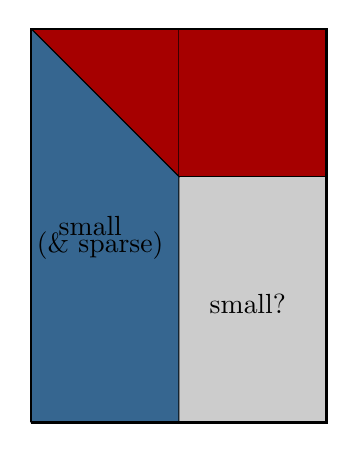
\begin{tikzpicture}[scale=0.25]
\draw[fill=black!20!white] (0,0) -- (0,20) -- ( 15,20) -- (15, 0) -- (0,0);
\draw[fill=white] (0,0) -- (0,20) -- (7.5,20) -- (7.5,0) -- (0,0);
\draw[fill=darkred] (0,20) -- (7.5,12.5) -- (7.5,20) -- (0,20);
\draw[fill=lightblue] (0,20) -- (7.5,12.5) -- (7.5,0) -- (0,0) -- (0,20);
\draw[fill=darkred] (7.5,20) -- (15,20) -- (15,12.5) -- (7.5,12.5);
\node[black] at (3,10) {small};
\node[black] at (3.5,9) {(\& sparse)};
\node[black] at (11,6) {small?};
\draw[thick] (0,0) -- (0,20) -- (15,20) -- (15, 0) -- (0,0);
\end{tikzpicture}\end{center}

\framebreak

We considering $a \approx \log n$ `blocks' of $b$ elements each.

\begin{equation*}
\left(
\begin{array}{cc|ccc|c}
\bold{a}_{11} & \bold{a}_{12} & \bold{a}_{13} & \cdots & \bold{a}_{1n} & c_0\\
\bold{a}_{21} & \bold{a}_{22} & \bold{a}_{23} & \cdots & \bold{a}_{2n} & c_1\\
\vdots & \vdots & \ddots & \vdots & \vdots\\
\bold{a}_{m1} & \bold{a}_{m2} & \bold{a}_{m3} & \cdots & \bold{a}_{mn} & c_{m}
\end{array}
\right)
\end{equation*}

\framebreak

For each block we build a table of all $q^b$ possible values indexed by $\Z_q^b$.

\begin{equation*}
T^0 = \left[ 
\begin{array}{ll|ccc|c}
-\lfloor\frac{q}{2}\rfloor & -\lfloor\frac{q}{2}\rfloor & \bold{t}_{13} & \cdots & \bold{t}_{1n} & c_{t,0}\\
-\lfloor\frac{q}{2}\rfloor & -\lfloor\frac{q}{2}\rfloor+1 & \bold{t}_{23} & \cdots & \bold{t}_{2n} & c_{t,1}\\
\phantom{--}\vdots & \phantom{--}\vdots & \ddots & \vdots & \vdots\\
\phantom{-}\lfloor\frac{q}{2}\rfloor & \phantom{-}\lfloor\frac{q}{2}\rfloor& \bold{t}_{q^23} & \cdots & \bold{t}_{q^2n} & c_{t,q^2}
\end{array}\right]
\end{equation*}

For each $\vec{z} \in \Z_q^b$ we try to find a row in $\vec{A}$ such that it contains $\vec{z}$ as a subvector at the target indices.

\framebreak

We use these tables to eliminate $b$ entries in other rows. Assume $(\vec{a}_{21},\vec{a}_{22}) = (\lfloor\frac{q}{2}\rfloor, \lfloor\frac{q}{2}\rfloor+1)$, then:

\begin{eqnarray*}
& & \left(
\begin{array}{cc|ccc|c}
\vec{a}_{11} & \vec{a}_{12} & \vec{a}_{13} & \cdots & \vec{a}_{1n} & c_0\\
\cemph{\vec{a}_{21}} & \cemph{\vec{a}_{22}} & \vec{a}_{23} & \cdots & \vec{a}_{2n} & c_1\\
\vdots & \vdots & \ddots & \vdots & \vdots\\
\vec{a}_{m1} & \vec{a}_{m2} & \vec{a}_{m3} & \cdots & \vec{a}_{mn} & c_{m}
\end{array}
\right)\\
&+& \left[
\begin{array}{ll|ccc|c}
-\lfloor\frac{q}{2}\rfloor & -\lfloor\frac{q}{2}\rfloor & \bold{t}_{13} & \cdots & \bold{t}_{1n} & c_{t,0}\\
\cemph{-\lfloor\frac{q}{2}\rfloor} & \cemph{-\lfloor\frac{q}{2}\rfloor+1} & \bold{t}_{23} & \cdots & \bold{t}_{2n} & c_{t,1}\\
\phantom{--}\vdots & \phantom{--}\vdots & \ddots & \vdots & \vdots\\
\phantom{-}\lfloor\frac{q}{2}\rfloor & \phantom{-}\lfloor\frac{q}{2}\rfloor& \bold{t}_{q^23} & \cdots & \bold{t}_{q^2n} & c_{t,q^2}
\end{array}\right]\\
&\Rightarrow& \left(
\begin{array}{cc|ccc|c}
\vec{a}_{11} & \vec{a}_{12} & \vec{a}_{13} & \cdots & \vec{a}_{1n} & c_0\\
\cemph{0} & \cemph{0} & \shortvec{a}_{23} & \cdots & \shortvec{a}_{2n} & \tilde{c}_1\\
\vdots & \vdots & \ddots & \vdots & \vdots\\
\vec{a}_{m1} & \vec{a}_{m2} & \vec{a}_{m3} & \cdots & \vec{a}_{mn} & c_{m}
\end{array}
\right)\phantom{\Longrightarrow}
\end{eqnarray*}

\framebreak
\begin{columns}
\column{0.6\textwidth} 


\begin{center}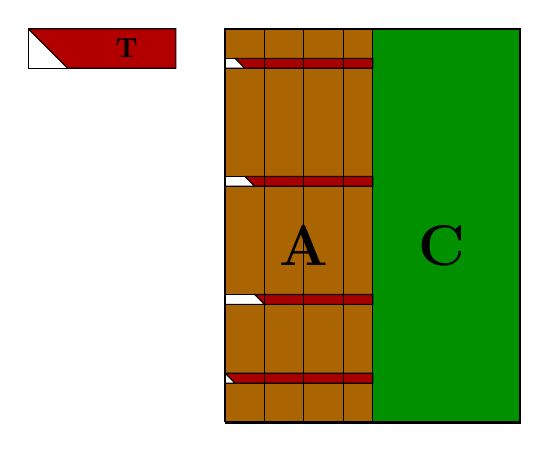
\begin{tikzpicture}[scale=0.25]
\draw[fill=darkgreen] (0,0) -- (0,20) -- (15,20) -- (15, 0) -- (0,0);
\draw[fill=lightbrown] (0,0) --(0,20) -- (7.5,20) -- (7.5,0) -- (0,0);
\draw[fill=white] (0, 2) --(0, 2.5) -- (7.5, 2.5) -- (7.5, 2) -- (0, 2);
\draw[fill=white] (0,18) --(0,18.5) -- (7.5,18.5) -- (7.5,18) -- (0,18);
\draw[fill=white] (0,12) --(0,12.5) -- (7.5,12.5) -- (7.5,12) -- (0,12);
\draw[fill=white] (0, 6) --(0, 6.5) -- (7.5, 6.5) -- (7.5, 6) -- (0, 6);

\draw[fill=darkred] (0.5, 2) --(0,   2.5) -- (7.5, 2.5) -- (7.5, 2) -- (0, 2);
\draw[fill=darkred] (1,  18) --(0.5,18.5) -- (7.5,18.5) -- (7.5,18) -- (0,18);
\draw[fill=darkred] (1.5,12) --(1  ,12.5) -- (7.5,12.5) -- (7.5,12) -- (0,12);
\draw[fill=darkred] (2, 6)  -- (1.5, 6.5) -- (7.5, 6.5) -- (7.5, 6) -- (0, 6);

\draw (2,0) -- (2,20);
\draw (4,0) -- (4,20);
\draw (6,0) -- (6,20);

\node at (4, 9) {\huge $\vec{A}$};
\node at (11, 9) {\huge $\vec{C}$};
\draw[thick] (0,0) -- (0,20) -- (15,20) -- (15, 0) -- (0,0);

\draw[fill=white] (-10,20) -- (-10,18) -- (-2.5,18) -- (-2.5,20) -- (-10,20);
\draw[fill=red!70!black] (-10,20) -- (-8,18) -- (-2.5,18)  -- (-2.5,20) -- (-10,20);
\node at (-5, 19) {$\vec{T}$};

\end{tikzpicture}\end{center}
\column{0.4\textwidth}
This is similar to Gaussian elimination with Gray code tables. There we construct the table $\vec{T}$ to reduce the number of vector additions. However, in the BKW case we find the table $\vec{T}$ in our matrix $\vec{A}$ instead of computing it by linear combinations of rows in $\vec{A}$.
\end{columns}

\vspace{1em}

One addition and no multiplications for clearing $b$ columns.

\framebreak

This gives a memory requirement of $$\approx\frac{q^b}{2}\cdot a\cdot(n+1)$$ and a time complexity of $$\approx (a^2n)\cdot\frac{q^b}{2}.$$

\vspace{1em}

A detailed analysis of the algorithm for LWE is available as:

\begin{thebibliography}{foobar}
\bibitem{foobar}
Martin R.\ Albrecht, Carlos Cid, Jean-Charles Faugère, Robert Fitzpatrick and Ludovic Perret
\newblock On the Complexity of the BKW Algorithm on LWE
\newblock {\em ePrint Report} 2012/636, 2012.
\newblock to appear in {\em Designs, Codes and Cryptography}.
\end{thebibliography}
\end{frame}

\section{Solving Decision-LWE with Small Secrets}

\begin{frame}
\frametitle{The Setting}

Assume $\vec{s} \sample \U{\Z_2^n}$, i.e.\ all entries in secret $\vec{s}$ are very small.

\vspace{1em}

This is a common setting in cryptography for performance reasons and because this allows to realise some advanced schemes. In particular, a technique called `modulus switching' can be used to improve the performance of homomorphic encryption schemes.

\vspace{1em}

\begin{thebibliography}{foobar}
\bibitem{brakerski-vaikuntanathan:focs2011}
Zvika Brakerski and Vinod Vaikuntanathan.
\newblock Efficient fully homomorphic encryption from (standard) {LWE}.
\newblock In Rafail Ostrovsky, editor, {\em IEEE 52nd Annual Symposium on
  Foundations of Computer Science, FOCS 2011}, pages 97--106. IEEE, 2011.
\end{thebibliography}

\end{frame}

\begin{frame}[allowframebreaks]
\frametitle{Modulus Reduction}

Given a sample $(\vec{a},c)$ where $c = \dotp{\vec{a}}{\vec{s}} + e$ and some $p < q $ we may consider $$\left(\round{\frac{p}{q} \cdot \vec{a}}, \round{\frac{p}{q} \cdot c}\right)$$ with
\begin{eqnarray*}
\round{\frac{p}{q} \cdot c} &=& \round{ \dotp{ \frac{p}{q} \cdot \vec{a} }{\vec{s} } + \frac{p}{q} \cdot e}\\
  &=& \round{ \dotp{ \round{ \frac{p}{q} \cdot \vec{a} }}{\vec{s} } + \dotp{\frac{p}{q} \cdot \vec{a} - \round{ \frac{p}{q} \cdot \vec{a} }}{\vec{s}} + \frac{p}{q} \cdot e}\\
  &=& \dotp{ \round{ \frac{p}{q} \cdot \vec{a} }}{\vec{s} } + \dotp{\frac{p}{q} \cdot \vec{a} - \round{ \frac{p}{q} \cdot \vec{a} }}{\vec{s}} + \frac{p}{q} \cdot e \pm [0,0.5]\\
  &=& \dotp{ \round{ \frac{p}{q} \cdot \vec{a} }}{\vec{s} } + e''.\\
\end{eqnarray*}

\framebreak

\begin{exampleblock}{Example}
\begin{eqnarray*}
p, q &=& 10, 20\\
\vec{a} &=& (8, -2, 0, 4, 2, -7),\\
\vec{s} &=& (0, 1, 0, 0, 1, 1),\\
 \dotp{\vec{a}}{\vec{s}} &=& -7,\\
c &=& -6\\
\vec{a'} = \round{\frac{p}{q} \cdot \vec{a}} &=& (4, -1, 0, 2, 1, -4)\\
\dotp{\vec{a'}}{\vec{s}} &=& -4,\\
\round{\frac{p}{q} \cdot c} &=& -4.\\
\end{eqnarray*}
\end{exampleblock}


\framebreak

Typically, we would choose

$$p \approx q \cdot \sqrt{n \cdot \Var(\U{[-0.5,0.5]}) \cdot \sigma^2_s}/\sigma = q \cdot \sqrt{n/12} \sigma_s/\sigma$$ where $\sigma_s$ is the standard deviation of elements in $\vec{s}$.

\vspace{1em}

If $\vec{s}$ is small then $e''$ is small and we may compute with the smaller `precision' $p$ at the cost of a slight increase of the noise rate. 

\vspace{1em}

The complexity hence drops to $$\approx (a^2n)\cdot\frac{p^b}{2}$$ with $a$ usually is unchanged.
\end{frame}

\begin{frame}[allowframebreaks,fragile]
\frametitle{Lazy Modulus Switching} 
For simplicity assume $p = 2^\kappa$ and consider the LWE matrix
\begin{eqnarray*}
\footnotesize
[\vec{A} \mid \vec{c}] &=& \left(\begin{array}{ccccc}
       \vec{a}_{1,1} & \vec{a}_{1,2} & \hspace{2em} \dots \hspace{2em} & \vec{a}_{1,n} & c_1\\
       \vec{a}_{2,1} & \vec{a}_{2,2} & \dots & \vec{a}_{2,n} & c_2\\
        \vdots & \vdots & \ddots & \vdots & \vdots\\
       \vec{a}_{m,1} & \vec{a}_{m,2} & \dots & \vec{a}_{m,n} & c_{m}\\
      \end{array}\right)\\
\end{eqnarray*}
as
\begin{eqnarray*}
\footnotesize
[\vec{A} \mid \vec{c}] & = & \left(\begin{array}{cccccccc}
       \vec{a}_{1,1}^h & \vec{a}_{1,1}^{l} \hspace{1em} & \vec{a}_{1,2}^h & \vec{a}_{1,2}^{l} & \hspace{1em} \dots \hspace{1em} & \vec{a}_{1,n}^h & \vec{a}_{1,n}^{l}  \hspace{1em} & c_1\\
       \vec{a}_{2,1}^h & \vec{a}_{2,1}^{l} \hspace{1em} & \vec{a}_{2,2}^h & \vec{a}_{2,2}^{l} & \hspace{1em} \dots \hspace{1em} & \vec{a}_{2,n}^h & \vec{a}_{2,n}^{l}  \hspace{1em} & c_2\\
        \vdots & \vdots & \vdots & \vdots & \ddots & \vdots & \vdots & \vdots\\
       \vec{a}_{m,1}^h & \vec{a}_{m,1}^{l} \hspace{1em} & \vec{a}_{m,2}^h & \vec{a}_{m,2}^{l} & \hspace{1em} \dots \hspace{1em} & \vec{a}_{m,n}^h & \vec{a}_{m,n}^{l}  \hspace{1em} & c_{m}\\
      \end{array}\right)\\
\end{eqnarray*}
where $\vec{a}_{i,j}^h$ and $\vec{a}_{i,j}^{l}$ denote high and low order bits:
\begin{itemize}
 \item $\vec{a}_{i,j}^h$ corresponds to $\round{p/q \cdot \vec{a}_{i,j}}$ and 
 \item $\vec{a}_{i,j}^l$ corresponds to $\round{p/q \cdot \vec{a}_{i,j}} - p/q \cdot \vec{a}_{i,j}$, the rounding error.
\end{itemize}

In order to clear the most significant bits in every component of the $\vec{a}_{i}$, we run the BKW algorithm on the matrix $[\vec{A} \mid \vec{c}]$ but only consider
\begin{eqnarray*}
[\vec{A},\vec{c}]^h &:=& \left(\begin{array}{ccccc}
       \vec{a}_{1,1}^h & \vec{a}_{1,2}^h & \hspace{2em} \dots \hspace{2em} & \vec{a}_{1,n}^h & c_1\\
       \vec{a}_{2,1}^h & \vec{a}_{2,2}^h & \dots & \vec{a}_{2,n}^h & c_2\\
        \vdots & \vdots & \ddots & \vdots & \vdots\\
       \vec{a}_{m,1}^h & \vec{a}_{m,2}^h & \dots & \vec{a}_{m,n}^h & c_{m}\\
      \end{array}\right),
\end{eqnarray*}
i.e.\ the ``higher order bits'', when searching for collisions. 

\vspace{1em}

We only manage elimination tables for the most significant $\kappa$ bits.

All arithmetic is performed in $\Zq$ but collisions are searched for in $\Zp$.

\framebreak

\begin{exampleblock}{Example}
Let $q,p = 16,8$ and let $\vec{a} = (-3,2,4) \in \Zq^3$. 

\vspace{1em}

Instead of searching for a vector $\vec{v} = (\pm3,\cdot,\cdot)$ we ignore the least significant bit. 

\vspace{1em}

Hence, both $(\pm 3,\cdot,\cdot)$ and $(\pm 2,\cdot,\cdot)$ will do.

\vspace{1em}

As a consequence we don't necessarily produce a vector $(0, \cdot, \cdot)$ after elimination, but one of $(0, \cdot, \cdot)$ or $(1, \cdot, \cdot)$, i.e.\ the first component is small.
\end{exampleblock}

\begin{block}{Analogy}
An analogy would be linear algebra with floating point numbers, where we define a tolerance when a small number counts as zero. We don't check \verb|x == 0| but \verb|abs(x) < tolerance|. The smaller $p$ the bigger this tolerance.
\end{block}

\framebreak

BKW without lazy modulus switching:
\begin{center}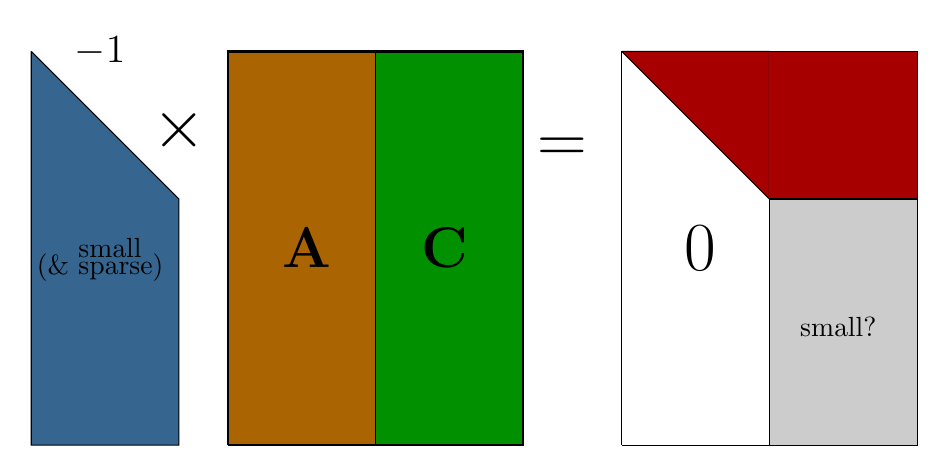
\begin{tikzpicture}[scale=0.25]

\draw[fill=lightblue] (-10,20) -- (-2.5,12.5) -- (-2.5,0) -- (-10,0) -- (-10,20);

\draw[fill=darkgreen] (0,0) -- (0,20) -- (15,20) -- (15, 0) -- (0,0);
\draw[fill=lightbrown] (0,0) --(0,20) -- (7.5,20) -- (7.5,0) -- (0,0);
\node at (4, 10) {\huge $\vec{A}$};
\node at (11, 10) {\huge $\vec{C}$};
\draw[thick] (0,0) -- (0,20) -- (15,20) -- (15, 0) -- (0,0);

\node at (-2.5,16) {\Huge $\times$};
\node at (-6.5,20) {\Large ${-1}$};

\node at (17,15) {\Huge $=$};
\draw[fill=white] (20,0) -- (20,20) -- (27.5,20) -- (27.5, 0) -- (20,0);
\draw[fill=black!20!white] (27.5,0) -- (27.5,20) -- (35,20) -- (35, 0) -- (27.5,0);

\draw[fill=darkred] (20,20) -- (27.5,12.5) -- (27.5,20) -- (20,20);
\draw[fill=darkred] (27.5,20) -- (35,20) -- (35,12.5) -- (27.5,12.5);


\node[black] at (-6, 10) {small};
\node[black] at (-6.5,9) {(\& sparse)};
\node[black] at (31,6) {small?};
\node[black] at (24,10) {\Huge 0};
\end{tikzpicture}\end{center}

\framebreak

BKW with lazy modulus switching ($\shortvec{A} \times \vec{S} + \shortvec{E} = \shortvec{C}$):
\begin{center}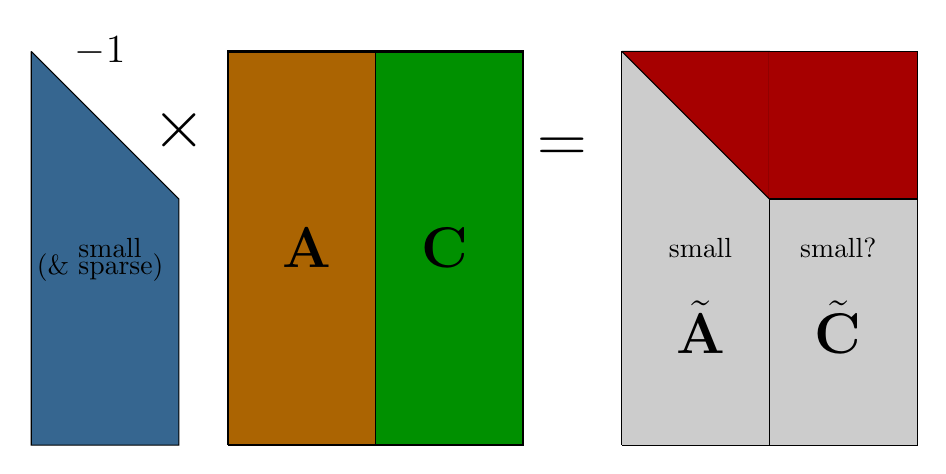
\begin{tikzpicture}[scale=0.25]

\draw[fill=lightblue] (-10,20) -- (-2.5,12.5) -- (-2.5,0) -- (-10,0) -- (-10,20);

\draw[fill=darkgreen] (0,0) -- (0,20) -- (15,20) -- (15, 0) -- (0,0);
\draw[fill=lightbrown] (0,0) --(0,20) -- (7.5,20) -- (7.5,0) -- (0,0);
\node at (4, 10) {\huge $\vec{A}$};
\node at (11, 10) {\huge $\vec{C}$};
\draw[thick] (0,0) -- (0,20) -- (15,20) -- (15, 0) -- (0,0);

\node at (-2.5,16) {\Huge $\times$};
\node at (-6.5,20) {\Large ${-1}$};

\node at (17,15) {\Huge $=$};
\draw[fill=black!20!white] (20,0) -- (20,20) -- (27.5,20) -- (27.5, 0) -- (20,0);
\draw[fill=black!20!white] (27.5,0) -- (27.5,20) -- (35,20) -- (35, 0) -- (27.5,0);

\draw[fill=darkred] (20,20) -- (27.5,12.5) -- (27.5,20) -- (20,20);
\draw[fill=darkred] (27.5,20) -- (35,20) -- (35,12.5) -- (27.5,12.5);


\node[black] at (-6, 10) {small};
\node[black] at (-6.5,9) {(\& sparse)};
\node[black] at (24,10) {small};
\node[black] at (31,10) {small?};

\node at (24,6) {\huge $\shortvec{A}$};
\node at (31,6) {\huge $\shortvec{C}$};

\end{tikzpicture}\end{center}

\framebreak

Difference to one-shot modulus reduction, i.e.\ rounding:
\begin{itemize}
 \item We do not apply modulus reduction in one shot, but only when needed. We compute with high precision but compare with low precision.
 \item As a consequence rounding errors accumulate not as fast: they only start to accumulate when we branch on a component.
\end{itemize}

\vspace{1em}

\begin{block}{}
\centering We may reduce $p$ by an additional factor of $\sqrt{a/2}$.
\end{block}

\end{frame}

\begin{frame}[allowframebreaks]
\frametitle{Complexity}


\textbf{BKW}
\begin{center}
\Large $\bigO{2^{cn}\cdot \polyfactor}$
\end{center}
\phantom{where $0<d\leq 1$  is a small constant.}\framebreak

\textbf{BKW + naive modulus switching}
\begin{center}
\Large $\bigO{2^{\big(c{\cemph +\frac{\log_2 d}{\log_2 n}}\big)\,n} \cdot \polyfactor}$
\end{center}
where $0<d\leq 1$  is a small constant (so $\log d < 0$).\framebreak


\textbf{BKW + lazy modulus switching}
\begin{center}
\Large $\bigO{2^{\big(c+\frac{\log_2 d{\cemph -\frac 1 2 \log_2 \log_2 n}}{\log_2 n}\big)\,n}\cdot \polyfactor}$
\end{center}
where $0<d\leq 1$  is a small constant.

\end{frame}

\subsection{A Heuristic Improvement}

\newcommand{\pivot}[4]{
\draw[fill=white]   (#1, #2) --(#1, #2+.5) -- (7.5, #2+.5) -- (7.5, #2) -- (#1, #2);
\draw[fill=darkred] (#3+0.5, #2) --(#3+0,   #2+.5) -- (7.5, #2+.5) -- (7.5, #2) -- (#3+0.5, #2);
\draw[fill=#4] (0,#2) -- (#1,#2) -- (#1,#2+.5) -- (0,#2+.5) -- (0,#2);
}

\begin{frame}[allowframebreaks,fragile]
\frametitle{The Problem}

We use the entries in Table $T^0$ to make the first $b$ components ``small''. However, as the algorithm proceeds we add up vectors with those small first $b$ components producing vectors where the first $b$ components are not that small any more. 

\framebreak


\begin{center}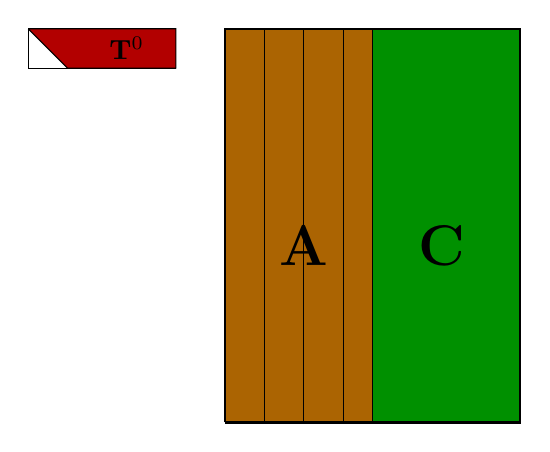
\begin{tikzpicture}[scale=0.25]
\draw[fill=darkgreen] (0,0) -- (0,20) -- (15,20) -- (15, 0) -- (0,0);
\draw[fill=lightbrown] (0,0) --(0,20) -- (7.5,20) -- (7.5,0) -- (0,0);
\pivot{0}{ 2}{0.0}{white};
\pivot{0}{ 6}{0.5}{white};
\pivot{0}{12}{1.0}{white};
\pivot{0}{18}{1.5}{white};

\draw (2,0) -- (2,20);
\draw (4,0) -- (4,20);
\draw (6,0) -- (6,20);

\node at (4, 9) {\huge $\vec{A}$};
\node at (11, 9) {\huge $\vec{C}$};
\draw[thick] (0,0) -- (0,20) -- (15,20) -- (15, 0) -- (0,0);

\draw[fill=white] (-10,20) -- (-10,18) -- (-2.5,18) -- (-2.5,20) -- (-10,20);
\draw[fill=red!70!black] (-10,20) -- (-8,18) -- (-2.5,18)  -- (-2.5,20) -- (-10,20);
\node at (-5, 19) {$\vec{T}^0$};

\end{tikzpicture}\end{center}

\framebreak

\begin{center}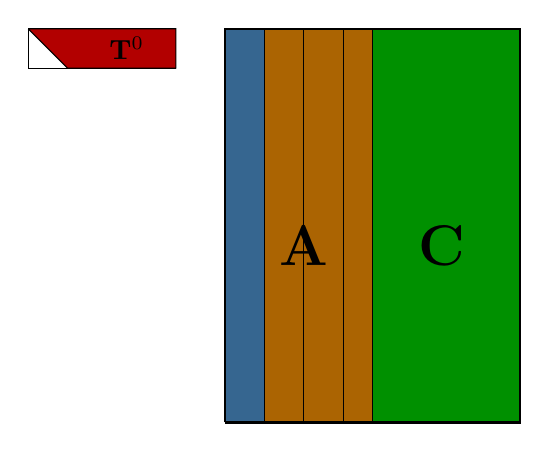
\begin{tikzpicture}[scale=0.25]
\draw[fill=darkgreen] (0,0) -- (0,20) -- (15,20) -- (15, 0) -- (0,0);
\draw[fill=lightbrown] (0,0) --(0,20) -- (7.5,20) -- (7.5,0) -- (0,0);
\draw[fill=lightblue] (0,0) --(0,20) -- (2,20) -- (2,0) -- (0,0);

\pivot{0}{ 2}{0.0}{white};
\pivot{0}{ 6}{0.5}{white};
\pivot{0}{12}{1.0}{white};
\pivot{0}{18}{1.5}{white};

\draw (2,0) -- (2,20);
\draw (4,0) -- (4,20);
\draw (6,0) -- (6,20);

\node at (4, 9) {\huge $\vec{A}$};
\node at (11, 9) {\huge $\vec{C}$};
\draw[thick] (0,0) -- (0,20) -- (15,20) -- (15, 0) -- (0,0);

\draw[fill=white] (-10,20) -- (-10,18) -- (-2.5,18) -- (-2.5,20) -- (-10,20);
\draw[fill=red!70!black] (-10,20) -- (-8,18) -- (-2.5,18)  -- (-2.5,20) -- (-10,20);
\node at (-5, 19) {$\vec{T}^0$};

\end{tikzpicture}\end{center}

\framebreak


\begin{center}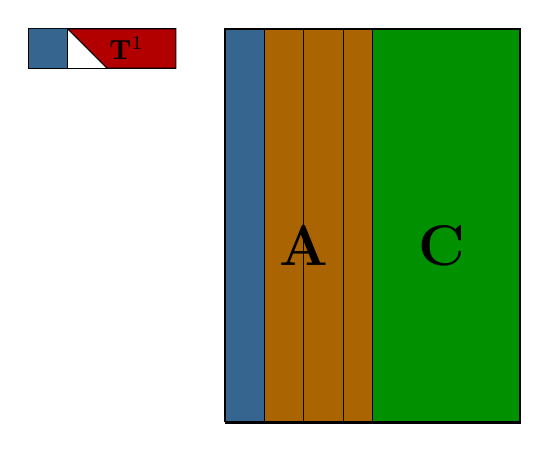
\begin{tikzpicture}[scale=0.25]
\draw[fill=darkgreen] (0,0) -- (0,20) -- (15,20) -- (15, 0) -- (0,0);
\draw[fill=lightbrown] (0,0) --(0,20) -- (7.5,20) -- (7.5,0) -- (0,0);
\draw[fill=lightblue] (0,0) --(0,20) -- (2,20) -- (2,0) -- (0,0);

\pivot{2}{ 1}{2.0}{lightblue};
\pivot{2}{ 3}{2.5}{lightblue};
\pivot{2}{ 7}{3.0}{lightblue};
\pivot{2}{13}{3.5}{lightblue};

\draw (2,0) -- (2,20);
\draw (4,0) -- (4,20);
\draw (6,0) -- (6,20);

\node at (4, 9) {\huge $\vec{A}$};
\node at (11, 9) {\huge $\vec{C}$};
\draw[thick] (0,0) -- (0,20) -- (15,20) -- (15, 0) -- (0,0);

\draw[fill=white] (-10,20) -- (-10,18) -- (-2.5,18) -- (-2.5,20) -- (-10,20);
\draw[fill=red!70!black] (-8,20) -- (-6,18) -- (-2.5,18)  -- (-2.5,20) -- (-8,20);
\draw[fill=lightblue] (-10,20) -- (-10,18) -- (-8,18) -- (-8,20) -- (-8,20);
\node at (-5, 19) {$\vec{T}^1$};

\end{tikzpicture}\end{center}


\framebreak

\begin{center}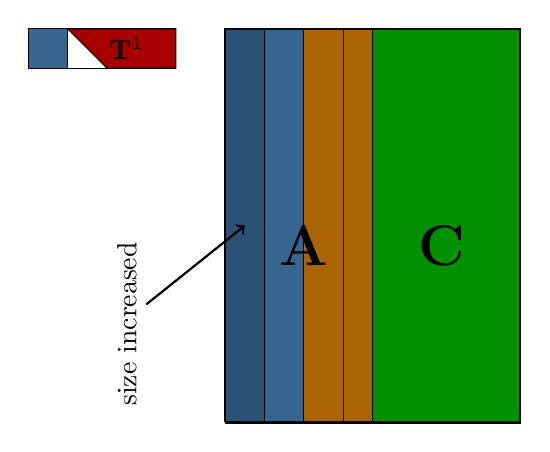
\begin{tikzpicture}[scale=0.25]
\draw[fill=darkgreen] (0,0) -- (0,20) -- (15,20) -- (15, 0) -- (0,0);
\draw[fill=lightbrown] (0,0) --(0,20) -- (7.5,20) -- (7.5,0) -- (0,0);
\draw[fill=lightblue!80!black] (0,0) --(0,20) -- (2,20) -- (2,0) -- (0,0);
\draw[fill=lightblue] (2,0) --(2,20) -- (4,20) -- (4,0) -- (2,0);

\pivot{2}{ 1}{2.0}{lightblue};
\pivot{2}{ 3}{2.5}{lightblue};
\pivot{2}{ 7}{3.0}{lightblue};
\pivot{2}{13}{3.5}{lightblue};

\draw (2,0) -- (2,20);
\draw (4,0) -- (4,20);
\draw (6,0) -- (6,20);

\node at (4, 9) {\huge $\vec{A}$};
\node at (11, 9) {\huge $\vec{C}$};
\draw[thick] (0,0) -- (0,20) -- (15,20) -- (15, 0) -- (0,0);

\draw[fill=white] (-10,20) -- (-10,18) -- (-2.5,18) -- (-2.5,20) -- (-10,20);
\draw[fill=darkred] (-8,20) -- (-6,18) -- (-2.5,18)  -- (-2.5,20) -- (-8,20);
\draw[fill=lightblue] (-10,20) -- (-10,18) -- (-8,18) -- (-8,20) -- (-8,20);
\node at (-5, 19) {$\vec{T}^1$};

\node[rotate=90] at (-5,5) {size increased};
\draw [->,thick] (-4,6) -- (1,10);

\end{tikzpicture}\end{center}


\framebreak

\begin{lemma}
\label{lem:regrowth}
Let $n\ge 1$ be the dimension of the LWE secret vector, $q$ be a modulus, $b \in \Z$ with $1 \leq b \le n$.   
Let also $\sigma_r$ be the standard deviation of uniformly random elements in $\Z_{\round{q/p}}$. Assuming all samples are independent, the components of $\shortvec{a} = \vec{a}- \vec{a}'$ returned by $\Bdis{\ell}$ satisfy:
$$
\Var(\shortvec{a}_{(i)}) = 2^{\ell - \lfloor i/b\rfloor} \sigma_r^2, \textnormal{ for } 0 \leq  \lfloor i/b \rfloor \leq \ell$$ and $\Var\big(\U{\Z_q}\big)$ for $\lfloor i/b\rfloor > \ell$.
\end{lemma}

\newcommand{\pvar}[3]{\draw[fill=lightblue] (#1-#2,-#3) -- (#1-#2,+#3) -- (#1+#2,+#3) -- (#1+#2,-#3) -- (#1-#2,-#3);}

\begin{center}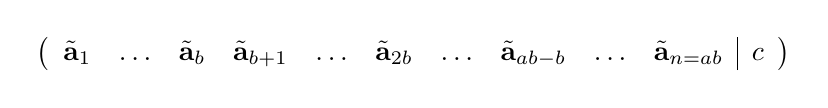
\begin{tikzpicture}
\pvar{-3.6}{1.0}{1.4}
\pvar{-1.15}{1.2}{0.7}
\pvar{2.55}{1.5}{0.35}
\pvar{4.45}{0.15}{1.6}
\node at (0,0) {$\left(\begin{array}{cccccccccc|c}\shortvec{a}_1 & \dots & \shortvec{a}_b  & \shortvec{a}_{b+1} & \dots &\shortvec{a}_{2b} &\dots &\shortvec{a}_{ab-b} & \dots & \shortvec{a}_{n=ab} & c\end{array}\right)$};

\end{tikzpicture}\end{center}

\end{frame}

\begin{frame}[allowframebreaks,fragile]
\frametitle{Unnatural Selection}

\begin{center}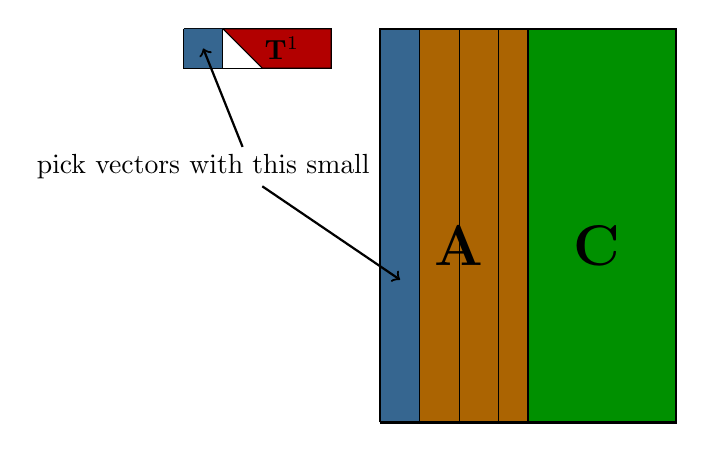
\begin{tikzpicture}[scale=0.25]
\draw[fill=darkgreen] (0,0) -- (0,20) -- (15,20) -- (15, 0) -- (0,0);
\draw[fill=lightbrown] (0,0) --(0,20) -- (7.5,20) -- (7.5,0) -- (0,0);
\draw[fill=lightblue] (0,0) --(0,20) -- (2,20) -- (2,0) -- (0,0);

\pivot{2}{ 1}{2.0}{lightblue};
\pivot{2}{ 3}{2.5}{lightblue};
\pivot{2}{ 7}{3.0}{lightblue};
\pivot{2}{13}{3.5}{lightblue};

\draw (2,0) -- (2,20);
\draw (4,0) -- (4,20);
\draw (6,0) -- (6,20);

\node at (4, 9) {\huge $\vec{A}$};
\node at (11, 9) {\huge $\vec{C}$};
\draw[thick] (0,0) -- (0,20) -- (15,20) -- (15, 0) -- (0,0);

\draw[fill=white] (-10,20) -- (-10,18) -- (-2.5,18) -- (-2.5,20) -- (-10,20);
\draw[fill=red!70!black] (-8,20) -- (-6,18) -- (-2.5,18)  -- (-2.5,20) -- (-8,20);
\draw[fill=lightblue] (-10,20) -- (-10,18) -- (-8,18) -- (-8,20) -- (-8,20);
\node at (-5, 19) {$\vec{T}^1$};

\node[] at (-9,13) {pick vectors with this small};
\draw [->,thick] (-7,14) -- (-9,19);
\draw [->,thick] (-6,12) -- (1,7.25);

\end{tikzpicture}\end{center}

\begin{block}{}
Finding vectors by chance with the first $bi-b$ components unusually small to populate $T^i$ is easier than finding vectors where the first $i$ components are unusally small.
\end{block}
\end{frame}

\begin{frame}[allowframebreaks]
\frametitle{Impact}

We keep sampling and pick that candidate vector $\vec{a}$ for index $\vec{z}$ in $\vec{T}^1$ where the first $b$ components are unusually small.

\vspace{1em}

$\Rightarrow$ We need to establish how much we can expect the size to drop if we sample a given number of times.

\framebreak

\begin{assumption}[Cowboy]
Let the vectors $\vec{x}_0,\ldots,\vec{x}_{n-1} \in \Z_q^{\tau}$ be sampled from some distribution $\mathcal{D}$ such that $\sigma^2 = \Var(\vec{x}_{i,(j)})$ where $\mathcal{D}$ is any distribution on (sub-)vectors observable in our algorithm. Let $\vec{x}^*=\min_{abs}\left(\vec{x}_0,\dots,\vec{x}_{n-1}\right)$ where $\min_{abs}$ picks that vector $\vec{x}^*$ with 
$\sum_{j=0}^{b\cdot\ell-1} \abs{\vec{x}^*_{(j)}}$ minimal. The standard deviation $\sigma_{n} = \sqrt{\Var(\vec{x}^*_{(0)})}=\cdots=\sqrt{\Var(\vec{x}^*_{(\tau-1)})}$ of components in $\vec{x}^*$ satisfies
$$\sigma/\sigma_n \geq c_\tau\, \sqrt[\tau]{n} + (1 - c_\tau)$$ with 
$$c_\tau \approx \frac{1}{5}\sqrt{\tau} + \frac{1}{3}.$$
\end{assumption}

\framebreak

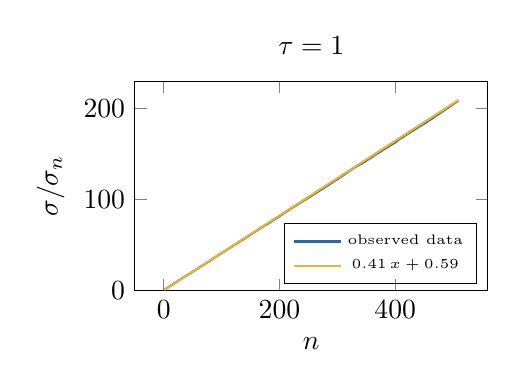
\begin{tikzpicture}
\pgfplotsset{width=.5\textwidth, height=0.35\textwidth}
\begin{axis}[xlabel={$n$},ylabel={$\sigma/\sigma_n$},ymin=0,legend pos=south east,title={$\tau=1$}, legend style={fill=none}]
\addplot[lightblue, thick] coordinates {
(  1, 1.00) (  5, 2.65) (  9, 4.28) ( 13, 5.92) ( 17, 7.54) ( 21, 9.19) ( 25, 10.83) ( 29, 12.47) ( 33, 14.12) ( 37, 15.74) ( 41, 17.29) ( 45, 18.85) ( 49, 20.47) ( 53, 22.09) ( 57, 23.66) ( 61, 25.26) ( 65, 26.90) ( 69, 28.51) ( 73, 30.15) ( 77, 31.68) ( 81, 33.40) ( 85, 35.10) ( 89, 36.76) ( 93, 38.42) ( 97, 40.08) (101, 41.65) (105, 43.30) (109, 44.88) (113, 46.45) (117, 48.11) (121, 49.75) (125, 51.44) (129, 52.95) (133, 54.59) (137, 56.11) (141, 57.80) (145, 59.43) (149, 61.10) (153, 62.87) (157, 64.42) (161, 65.98) (165, 67.66) (169, 69.38) (173, 70.93) (177, 72.38) (181, 73.84) (185, 75.44) (189, 77.15) (193, 78.82) (197, 80.39) (201, 82.06) (205, 83.86) (209, 85.52) (213, 87.10) (217, 88.90) (221, 90.51) (225, 92.10) (229, 93.56) (233, 95.28) (237, 96.95) (241, 98.50) (245, 99.97) (249, 101.53) (253, 103.17) (257, 104.83) (261, 106.45) (265, 107.99) (269, 109.59) (273, 111.15) (277, 112.88) (281, 114.50) (285, 116.00) (289, 117.74) (293, 119.46) (297, 121.11) (301, 122.61) (305, 124.36) (309, 126.10) (313, 127.76) (317, 129.59) (321, 131.37) (325, 133.03) (329, 134.78) (333, 136.20) (337, 137.62) (341, 138.94) (345, 140.53) (349, 142.17) (353, 143.88) (357, 145.41) (361, 147.05) (365, 148.81) (369, 150.39) (373, 151.86) (377, 153.50) (381, 155.20) (385, 156.69) (389, 158.30) (393, 159.90) (397, 161.37) (401, 163.14) (405, 165.11) (409, 166.87) (413, 168.28) (417, 170.09) (421, 171.64) (425, 173.41) (429, 174.83) (433, 176.39) (437, 178.15) (441, 179.67) (445, 181.29) (449, 182.80) (453, 184.30) (457, 185.98) (461, 187.66) (465, 189.26) (469, 191.24) (473, 192.74) (477, 194.53) (481, 196.21) (485, 197.99) (489, 199.71) (493, 201.31) (497, 203.03) (501, 204.80) (505, 206.53) (509, 208.03)

};
\addlegendentry{{\tiny observed data}}
\addplot[yellow9,thick] coordinates {
(  1, 1.00) (  5, 2.64) (  9, 4.27) ( 13, 5.91) ( 17, 7.55) ( 21, 9.18) ( 25, 10.82) ( 29, 12.45) ( 33, 14.09) ( 37, 15.73) ( 41, 17.36) ( 45, 19.00) ( 49, 20.64) ( 53, 22.27) ( 57, 23.91) ( 61, 25.54) ( 65, 27.18) ( 69, 28.82) ( 73, 30.45) ( 77, 32.09) ( 81, 33.73) ( 85, 35.36) ( 89, 37.00) ( 93, 38.63) ( 97, 40.27) (101, 41.91) (105, 43.54) (109, 45.18) (113, 46.82) (117, 48.45) (121, 50.09) (125, 51.73) (129, 53.36) (133, 55.00) (137, 56.63) (141, 58.27) (145, 59.91) (149, 61.54) (153, 63.18) (157, 64.82) (161, 66.45) (165, 68.09) (169, 69.72) (173, 71.36) (177, 73.00) (181, 74.63) (185, 76.27) (189, 77.91) (193, 79.54) (197, 81.18) (201, 82.82) (205, 84.45) (209, 86.09) (213, 87.72) (217, 89.36) (221, 91.00) (225, 92.63) (229, 94.27) (233, 95.91) (237, 97.54) (241, 99.18) (245, 100.81) (249, 102.45) (253, 104.09) (257, 105.72) (261, 107.36) (265, 109.00) (269, 110.63) (273, 112.27) (277, 113.90) (281, 115.54) (285, 117.18) (289, 118.81) (293, 120.45) (297, 122.09) (301, 123.72) (305, 125.36) (309, 127.00) (313, 128.63) (317, 130.27) (321, 131.90) (325, 133.54) (329, 135.18) (333, 136.81) (337, 138.45) (341, 140.09) (345, 141.72) (349, 143.36) (353, 144.99) (357, 146.63) (361, 148.27) (365, 149.90) (369, 151.54) (373, 153.18) (377, 154.81) (381, 156.45) (385, 158.09) (389, 159.72) (393, 161.36) (397, 162.99) (401, 164.63) (405, 166.27) (409, 167.90) (413, 169.54) (417, 171.18) (421, 172.81) (425, 174.45) (429, 176.08) (433, 177.72) (437, 179.36) (441, 180.99) (445, 182.63) (449, 184.27) (453, 185.90) (457, 187.54) (461, 189.17) (465, 190.81) (469, 192.45) (473, 194.08) (477, 195.72) (481, 197.36) (485, 198.99) (489, 200.63) (493, 202.27) (497, 203.90) (501, 205.54) (505, 207.17) (509, 208.81)
};
\addlegendentry{{\tiny $0.41\, x + 0.59$}}
\end{axis}
\end{tikzpicture}
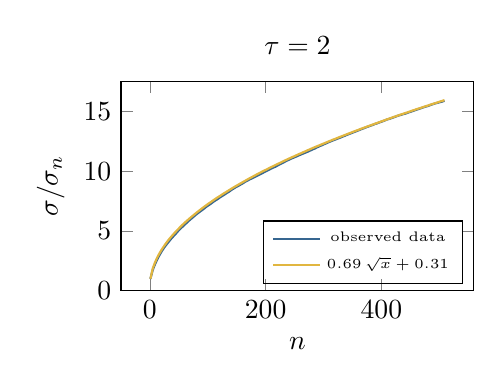
\begin{tikzpicture}
\pgfplotsset{width=.5\textwidth, height=0.35\textwidth}
\begin{axis}[xlabel={$n$},ylabel={$\sigma/\sigma_n$},ymin=0,legend pos=south east,title={$\tau=2$}, legend style={fill=none}]
\addplot[lightblue, thick] coordinates {
(  1, 1.00) (  5, 1.74) (  9, 2.23) ( 13, 2.65) ( 17, 3.01) ( 21, 3.34) ( 25, 3.63) ( 29, 3.88) ( 33, 4.12) ( 37, 4.36) ( 41, 4.57) ( 45, 4.78) ( 49, 5.00) ( 53, 5.20) ( 57, 5.38) ( 61, 5.56) ( 65, 5.74) ( 69, 5.92) ( 73, 6.08) ( 77, 6.25) ( 81, 6.41) ( 85, 6.56) ( 89, 6.70) ( 93, 6.84) ( 97, 7.00) (101, 7.13) (105, 7.26) (109, 7.41) (113, 7.54) (117, 7.66) (121, 7.80) (125, 7.92) (129, 8.04) (133, 8.17) (137, 8.29) (141, 8.43) (145, 8.55) (149, 8.67) (153, 8.77) (157, 8.88) (161, 8.99) (165, 9.12) (169, 9.22) (173, 9.32) (177, 9.41) (181, 9.51) (185, 9.60) (189, 9.70) (193, 9.80) (197, 9.90) (201, 10.00) (205, 10.10) (209, 10.20) (213, 10.29) (217, 10.37) (221, 10.48) (225, 10.58) (229, 10.68) (233, 10.78) (237, 10.88) (241, 10.97) (245, 11.06) (249, 11.14) (253, 11.22) (257, 11.31) (261, 11.39) (265, 11.47) (269, 11.55) (273, 11.63) (277, 11.72) (281, 11.81) (285, 11.89) (289, 11.99) (293, 12.08) (297, 12.16) (301, 12.25) (305, 12.33) (309, 12.42) (313, 12.50) (317, 12.58) (321, 12.65) (325, 12.73) (329, 12.80) (333, 12.88) (337, 12.96) (341, 13.04) (345, 13.12) (349, 13.19) (353, 13.27) (357, 13.34) (361, 13.42) (365, 13.50) (369, 13.57) (373, 13.65) (377, 13.72) (381, 13.79) (385, 13.86) (389, 13.94) (393, 14.00) (397, 14.08) (401, 14.14) (405, 14.22) (409, 14.30) (413, 14.36) (417, 14.42) (421, 14.49) (425, 14.56) (429, 14.64) (433, 14.69) (437, 14.75) (441, 14.80) (445, 14.87) (449, 14.94) (453, 15.00) (457, 15.07) (461, 15.14) (465, 15.20) (469, 15.27) (473, 15.34) (477, 15.40) (481, 15.45) (485, 15.53) (489, 15.60) (493, 15.66) (497, 15.71) (501, 15.76) (505, 15.81) (509, 15.88)
};
\addlegendentry{{\tiny observed data}}
\addplot[yellow9, thick] coordinates {
(  1, 1.00) (  5, 1.86) (  9, 2.38) ( 13, 2.80) ( 17, 3.16) ( 21, 3.48) ( 25, 3.77) ( 29, 4.04) ( 33, 4.29) ( 37, 4.52) ( 41, 4.74) ( 45, 4.95) ( 49, 5.15) ( 53, 5.35) ( 57, 5.54) ( 61, 5.72) ( 65, 5.89) ( 69, 6.06) ( 73, 6.22) ( 77, 6.38) ( 81, 6.54) ( 85, 6.69) ( 89, 6.84) ( 93, 6.99) ( 97, 7.13) (101, 7.27) (105, 7.40) (109, 7.54) (113, 7.67) (117, 7.80) (121, 7.92) (125, 8.05) (129, 8.17) (133, 8.29) (137, 8.41) (141, 8.53) (145, 8.65) (149, 8.76) (153, 8.87) (157, 8.98) (161, 9.09) (165, 9.20) (169, 9.31) (173, 9.42) (177, 9.52) (181, 9.62) (185, 9.73) (189, 9.83) (193, 9.93) (197, 10.03) (201, 10.12) (205, 10.22) (209, 10.32) (213, 10.41) (217, 10.51) (221, 10.60) (225, 10.69) (229, 10.79) (233, 10.88) (237, 10.97) (241, 11.06) (245, 11.15) (249, 11.23) (253, 11.32) (257, 11.41) (261, 11.49) (265, 11.58) (269, 11.66) (273, 11.75) (277, 11.83) (281, 11.92) (285, 12.00) (289, 12.08) (293, 12.16) (297, 12.24) (301, 12.32) (305, 12.40) (309, 12.48) (313, 12.56) (317, 12.64) (321, 12.71) (325, 12.79) (329, 12.87) (333, 12.94) (337, 13.02) (341, 13.09) (345, 13.17) (349, 13.24) (353, 13.32) (357, 13.39) (361, 13.46) (365, 13.54) (369, 13.61) (373, 13.68) (377, 13.75) (381, 13.82) (385, 13.89) (389, 13.96) (393, 14.03) (397, 14.10) (401, 14.17) (405, 14.24) (409, 14.31) (413, 14.38) (417, 14.45) (421, 14.52) (425, 14.58) (429, 14.65) (433, 14.72) (437, 14.78) (441, 14.85) (445, 14.91) (449, 14.98) (453, 15.05) (457, 15.11) (461, 15.18) (465, 15.24) (469, 15.30) (473, 15.37) (477, 15.43) (481, 15.49) (485, 15.56) (489, 15.62) (493, 15.68) (497, 15.74) (501, 15.81) (505, 15.87) (509, 15.93)
};
\addlegendentry{{\tiny $0.69\, \sqrt{x} + 0.31$}}
\end{axis}
\end{tikzpicture}\\
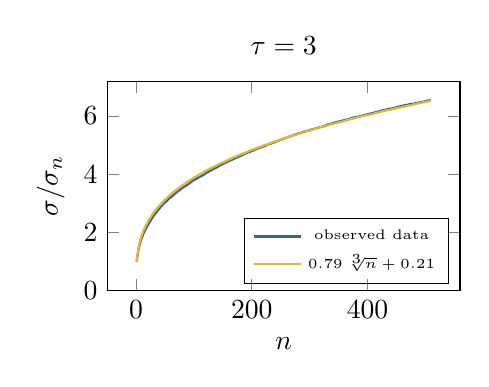
\begin{tikzpicture}
\pgfplotsset{width=.5\textwidth, height=0.35\textwidth}
\begin{axis}[xlabel={$n$},ylabel={$\sigma/\sigma_n$},ymin=0,legend pos=south east,title={$\tau=3$}, legend style={fill=none}]
\addplot[lightblue, thick] coordinates {
(  1, 1.00) (  5, 1.49) (  9, 1.76) ( 13, 1.97) ( 17, 2.13) ( 21, 2.27) ( 25, 2.40) ( 29, 2.53) ( 33, 2.64) ( 37, 2.74) ( 41, 2.84) ( 45, 2.93) ( 49, 3.01) ( 53, 3.08) ( 57, 3.16) ( 61, 3.22) ( 65, 3.29) ( 69, 3.36) ( 73, 3.42) ( 77, 3.48) ( 81, 3.54) ( 85, 3.59) ( 89, 3.64) ( 93, 3.70) ( 97, 3.76) (101, 3.81) (105, 3.85) (109, 3.90) (113, 3.94) (117, 3.98) (121, 4.04) (125, 4.08) (129, 4.13) (133, 4.17) (137, 4.21) (141, 4.25) (145, 4.30) (149, 4.34) (153, 4.38) (157, 4.42) (161, 4.46) (165, 4.49) (169, 4.53) (173, 4.56) (177, 4.60) (181, 4.63) (185, 4.67) (189, 4.71) (193, 4.74) (197, 4.77) (201, 4.80) (205, 4.84) (209, 4.87) (213, 4.90) (217, 4.93) (221, 4.96) (225, 4.99) (229, 5.03) (233, 5.05) (237, 5.08) (241, 5.11) (245, 5.14) (249, 5.17) (253, 5.20) (257, 5.23) (261, 5.26) (265, 5.29) (269, 5.31) (273, 5.35) (277, 5.37) (281, 5.40) (285, 5.42) (289, 5.45) (293, 5.47) (297, 5.49) (301, 5.52) (305, 5.54) (309, 5.56) (313, 5.58) (317, 5.61) (321, 5.63) (325, 5.65) (329, 5.69) (333, 5.71) (337, 5.73) (341, 5.76) (345, 5.78) (349, 5.80) (353, 5.82) (357, 5.84) (361, 5.86) (365, 5.88) (369, 5.90) (373, 5.93) (377, 5.95) (381, 5.96) (385, 5.98) (389, 6.00) (393, 6.02) (397, 6.04) (401, 6.06) (405, 6.08) (409, 6.10) (413, 6.12) (417, 6.14) (421, 6.16) (425, 6.19) (429, 6.20) (433, 6.22) (437, 6.24) (441, 6.25) (445, 6.27) (449, 6.29) (453, 6.31) (457, 6.33) (461, 6.35) (465, 6.37) (469, 6.38) (473, 6.40) (477, 6.41) (481, 6.43) (485, 6.44) (489, 6.46) (493, 6.48) (497, 6.49) (501, 6.51) (505, 6.53) (509, 6.54)
};
\addlegendentry{{\tiny observed data}}
\addplot[yellow9, thick] coordinates {
(  1, 1.00) (  5, 1.56) (  9, 1.85) ( 13, 2.07) ( 17, 2.24) ( 21, 2.39) ( 25, 2.52) ( 29, 2.64) ( 33, 2.74) ( 37, 2.84) ( 41, 2.93) ( 45, 3.02) ( 49, 3.10) ( 53, 3.18) ( 57, 3.25) ( 61, 3.32) ( 65, 3.39) ( 69, 3.45) ( 73, 3.51) ( 77, 3.57) ( 81, 3.63) ( 85, 3.68) ( 89, 3.74) ( 93, 3.79) ( 97, 3.84) (101, 3.89) (105, 3.94) (109, 3.98) (113, 4.03) (117, 4.07) (121, 4.12) (125, 4.16) (129, 4.20) (133, 4.24) (137, 4.28) (141, 4.32) (145, 4.36) (149, 4.40) (153, 4.43) (157, 4.47) (161, 4.51) (165, 4.54) (169, 4.58) (173, 4.61) (177, 4.65) (181, 4.68) (185, 4.71) (189, 4.74) (193, 4.77) (197, 4.81) (201, 4.84) (205, 4.87) (209, 4.90) (213, 4.93) (217, 4.96) (221, 4.99) (225, 5.01) (229, 5.04) (233, 5.07) (237, 5.10) (241, 5.13) (245, 5.15) (249, 5.18) (253, 5.21) (257, 5.23) (261, 5.26) (265, 5.28) (269, 5.31) (273, 5.33) (277, 5.36) (281, 5.38) (285, 5.41) (289, 5.43) (293, 5.46) (297, 5.48) (301, 5.50) (305, 5.53) (309, 5.55) (313, 5.57) (317, 5.60) (321, 5.62) (325, 5.64) (329, 5.66) (333, 5.69) (337, 5.71) (341, 5.73) (345, 5.75) (349, 5.77) (353, 5.79) (357, 5.81) (361, 5.83) (365, 5.86) (369, 5.88) (373, 5.90) (377, 5.92) (381, 5.94) (385, 5.96) (389, 5.98) (393, 6.00) (397, 6.02) (401, 6.03) (405, 6.05) (409, 6.07) (413, 6.09) (417, 6.11) (421, 6.13) (425, 6.15) (429, 6.17) (433, 6.19) (437, 6.20) (441, 6.22) (445, 6.24) (449, 6.26) (453, 6.28) (457, 6.29) (461, 6.31) (465, 6.33) (469, 6.35) (473, 6.36) (477, 6.38) (481, 6.40) (485, 6.42) (489, 6.43) (493, 6.45) (497, 6.47) (501, 6.48) (505, 6.50) (509, 6.52)
};
\addlegendentry{{\tiny $0.79\, \sqrt[3]{n} +  0.21$}}
\end{axis}
\end{tikzpicture}
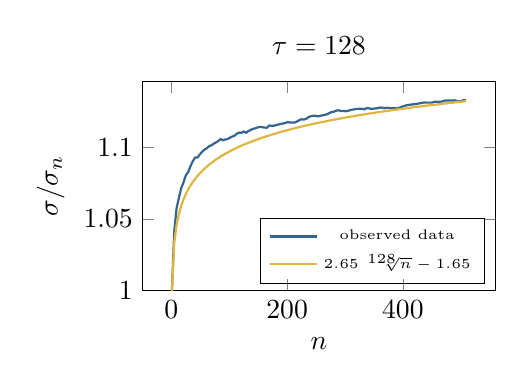
\begin{tikzpicture}
\pgfplotsset{width=.5\textwidth, height=0.35\textwidth}
\begin{axis}[xlabel={$n$},ylabel={$\sigma/\sigma_n$},ymin=1,legend pos=south east,title={$\tau=128$}, legend style={fill=none}]
\addplot[lightblue, thick] coordinates {
(  1, 1.0000) (  5, 1.0418) (  9, 1.0575) ( 13, 1.0648) ( 17, 1.0715) ( 21, 1.0755) ( 25, 1.0804) ( 29, 1.0827) ( 33, 1.0868) ( 37, 1.0902) ( 41, 1.0928) ( 45, 1.0928) ( 49, 1.0949) ( 53, 1.0968) ( 57, 1.0983) ( 61, 1.0992) ( 65, 1.1007) ( 69, 1.1013) ( 73, 1.1024) ( 77, 1.1033) ( 81, 1.1043) ( 85, 1.1057) ( 89, 1.1049) ( 93, 1.1054) ( 97, 1.1057) (101, 1.1066) (105, 1.1074) (109, 1.1080) (113, 1.1094) (117, 1.1102) (121, 1.1100) (125, 1.1109) (129, 1.1101) (133, 1.1113) (137, 1.1120) (141, 1.1128) (145, 1.1132) (149, 1.1138) (153, 1.1142) (157, 1.1140) (161, 1.1137) (165, 1.1136) (169, 1.1151) (173, 1.1150) (177, 1.1149) (181, 1.1155) (185, 1.1158) (189, 1.1162) (193, 1.1166) (197, 1.1169) (201, 1.1176) (205, 1.1172) (209, 1.1173) (213, 1.1172) (217, 1.1179) (221, 1.1189) (225, 1.1195) (229, 1.1193) (233, 1.1198) (237, 1.1210) (241, 1.1216) (245, 1.1220) (249, 1.1220) (253, 1.1215) (257, 1.1219) (261, 1.1222) (265, 1.1226) (269, 1.1230) (273, 1.1238) (277, 1.1246) (281, 1.1248) (285, 1.1255) (289, 1.1258) (293, 1.1252) (297, 1.1253) (301, 1.1251) (305, 1.1253) (309, 1.1259) (313, 1.1262) (317, 1.1265) (321, 1.1267) (325, 1.1268) (329, 1.1268) (333, 1.1264) (337, 1.1272) (341, 1.1272) (345, 1.1267) (349, 1.1269) (353, 1.1270) (357, 1.1273) (361, 1.1277) (365, 1.1275) (369, 1.1272) (373, 1.1275) (377, 1.1273) (381, 1.1272) (385, 1.1273) (389, 1.1270) (393, 1.1274) (397, 1.1280) (401, 1.1286) (405, 1.1291) (409, 1.1295) (413, 1.1296) (417, 1.1299) (421, 1.1300) (425, 1.1303) (429, 1.1306) (433, 1.1309) (437, 1.1312) (441, 1.1311) (445, 1.1311) (449, 1.1311) (453, 1.1314) (457, 1.1318) (461, 1.1317) (465, 1.1316) (469, 1.1321) (473, 1.1325) (477, 1.1326) (481, 1.1326) (485, 1.1325) (489, 1.1327) (493, 1.1323) (497, 1.1318) (501, 1.1322) (505, 1.1328) (509, 1.1327)
};
\addlegendentry{{\tiny observed data}}
\addplot[yellow9, thick] coordinates {
(  1, 1.0000) (  5, 1.0335) (  9, 1.0458) ( 13, 1.0536) ( 17, 1.0592) ( 21, 1.0637) ( 25, 1.0674) ( 29, 1.0706) ( 33, 1.0733) ( 37, 1.0757) ( 41, 1.0779) ( 45, 1.0799) ( 49, 1.0817) ( 53, 1.0834) ( 57, 1.0849) ( 61, 1.0864) ( 65, 1.0878) ( 69, 1.0890) ( 73, 1.0902) ( 77, 1.0914) ( 81, 1.0925) ( 85, 1.0935) ( 89, 1.0945) ( 93, 1.0954) ( 97, 1.0963) (101, 1.0972) (105, 1.0980) (109, 1.0988) (113, 1.0996) (117, 1.1003) (121, 1.1011) (125, 1.1018) (129, 1.1024) (133, 1.1031) (137, 1.1037) (141, 1.1043) (145, 1.1050) (149, 1.1055) (153, 1.1061) (157, 1.1067) (161, 1.1072) (165, 1.1077) (169, 1.1082) (173, 1.1087) (177, 1.1092) (181, 1.1097) (185, 1.1102) (189, 1.1107) (193, 1.1111) (197, 1.1115) (201, 1.1120) (205, 1.1124) (209, 1.1128) (213, 1.1132) (217, 1.1136) (221, 1.1140) (225, 1.1144) (229, 1.1148) (233, 1.1152) (237, 1.1155) (241, 1.1159) (245, 1.1163) (249, 1.1166) (253, 1.1169) (257, 1.1173) (261, 1.1176) (265, 1.1179) (269, 1.1183) (273, 1.1186) (277, 1.1189) (281, 1.1192) (285, 1.1195) (289, 1.1198) (293, 1.1201) (297, 1.1204) (301, 1.1207) (305, 1.1210) (309, 1.1213) (313, 1.1215) (317, 1.1218) (321, 1.1221) (325, 1.1224) (329, 1.1226) (333, 1.1229) (337, 1.1231) (341, 1.1234) (345, 1.1237) (349, 1.1239) (353, 1.1241) (357, 1.1244) (361, 1.1246) (365, 1.1249) (369, 1.1251) (373, 1.1253) (377, 1.1256) (381, 1.1258) (385, 1.1260) (389, 1.1262) (393, 1.1265) (397, 1.1267) (401, 1.1269) (405, 1.1271) (409, 1.1273) (413, 1.1275) (417, 1.1278) (421, 1.1280) (425, 1.1282) (429, 1.1284) (433, 1.1286) (437, 1.1288) (441, 1.1290) (445, 1.1292) (449, 1.1294) (453, 1.1296) (457, 1.1297) (461, 1.1299) (465, 1.1301) (469, 1.1303) (473, 1.1305) (477, 1.1307) (481, 1.1309) (485, 1.1310) (489, 1.1312) (493, 1.1314) (497, 1.1316) (501, 1.1317) (505, 1.1319) (509, 1.1321)
};
\addlegendentry{{\tiny $2.65\,\sqrt[128]{n} -1.65$}}
\end{axis}
\end{tikzpicture}


\end{frame}

\section{Results}

\begin{frame}[allowframebreaks]
\frametitle{BKW Variants}

\begin{table}[htbp]
\footnotesize
\centering
\begin{tabular}{|r||r|r||r|r|}
\hline
    & \multicolumn{2}{|c||}{BKW} & \multicolumn{2}{|c|}{+ Mod.\ Switch}\\
\hline
$n$ & $\log \Z_2$ & $\log \textnormal{mem}$ &$\log \Z_2$ & $\log \textnormal{mem}$\\
\hline
 128 &   97.6 &   90.0  &   89.6 &   81.2\\
 256 &  182.1 &  174.2  &  164.0 &  156.7\\
 512 &  361.0 &  352.8  &  305.6 &  297.9\\
1024 &  705.5 &  697.0  &  580.2 &  572.2\\
2048 & 1388.7 & 1379.9  & 1153.6 & 1145.3\\

\hline
    & \multicolumn{2}{|c||}{This Work (1)} & \multicolumn{2}{|c|}{This Work (2)}\\
\hline
$n$ & $\log \Z_2$ & $\log \textnormal{mem}$ &$\log \Z_2$ & $\log \textnormal{mem}$\\
\hline
 128 &  78.2 &  70.8 &  74.2 &  46.3\\
 256 & 142.7 & 134.9 & 132.5 &  67.1\\
 512 & 251.2 & 243.1 & 241.8 & 180.0\\
1024 & 494.8 & 486.5 & 485.0 & 407.5\\
2048 & 916.4 & 907.9 & 853.2 & 758.9\\
\hline
\end{tabular}
\caption{Cost for solving Decision-LWE with advantage $\approx 1$ for BKW and BKZ variants where $q$ and $\sigma$ are chosen as in Regev's scheme and $\vec{s} \sample \U{\Z_2^n}$ ``$\log \Z_2$'' gives the number of ``bit operations'' and ``$\log \textnormal{mem}$'' the memory requirement of $\Zq$ elements. All logarithms are base 2.}
\label{tab:modred}
\end{table}

\framebreak

\begin{tikzpicture}
\begin{axis}[xlabel={$\log_2 n$},ylabel={$\log_2$ speedup wrt BKW},ymin=0,legend pos=south west,title={$\log_2 \Z_2$ for $\vec{s} \sample \U{\{0,1\}}^n$}, legend style={fill=none}]
\addplot[yellow9,very thick] coordinates {
( 5,   40.0/  40.0) 
( 6,   55.9/  55.9) 
( 7,   97.6/  97.6) 
( 8,  182.1/ 182.1) 
( 9,  361.0/ 361.0) 
(10,  705.5/ 705.5) 
(11, 1388.7/1388.7) };
\addlegendentry{BKW};

\addplot[orange,very thick] coordinates {
( 5,   40.0/  39.4)
( 6,   55.9/  52.5)
( 7,   97.6/  89.6)
( 8,  182.1/ 164.0)
( 9,  361.0/ 305.6)
(10,  705.5/ 580.2)
(11, 1388.7/1153.6) };
\addlegendentry{BKW w/ modulus switching};


\addplot[darkred,thick] coordinates {  };
\addlegendentry{this work w/o unnatural selection};

\addplot[lightblue,very thick] coordinates { 
( 5,   40.0/ 40.00)
( 6,   55.9/ 49.20)
( 7,   97.6/ 78.20)
( 8,  182.1/142.70)
( 9,  361.0/251.20)
(10,  705.5/494.80)
(11, 1388.7/916.40)
 };
\addlegendentry{this work w/ unnatural selection};

\addplot[darkgreen,very thick] coordinates {
( 5,   40.0/ 40.00) 
( 6,   55.9/ 47.60)  
( 7,   97.6/ 74.20)
( 8,  182.1/132.50)
( 9,  361.0/241.80)
(10,  705.5/485.00)
(11, 1388.7/853.20)};
\addlegendentry{this work w/ unnatural selection};
\end{axis}
\end{tikzpicture}

\end{frame}



\begin{frame}[allowframebreaks]
\frametitle{\dots and Previous Work}

\begin{description}
 \item[MITM] guess the two halfes of the secret and search for a collision
 \item[BKZ] solve SIS using the BKZ algorithm with $\log_2 T_{sec} = 1.8/\log_2 \delta_0 - 110$.
 \item[BKZ 2] solve SIS using the BKZ algorithm with $\log_2 T_{sec} = 0.009/\log^2_2 \delta_0 - 27$.
\end{description}

\begin{thebibliography}{foo}
\bibitem{chen-nguyen:asiacrypt2011}
Yuanmi Chen and Phong~Q. Nguyen.
\newblock {BKZ} 2.0: better lattice security estimates.
\newblock In {\em Advances in Cryptology - ASIACRYPT 2011}, volume 7073 of {\em
  Lecture Notes in Computer Science}, pages 1--20, Berlin, Heidelberg, 2011.
  Springer Verlag.

\bibitem{LindnerP10}
Richard Lindner and Chris Peikert.
\newblock Better key sizes (and attacks) for {LWE}-based encryption.
\newblock In {\em Topics in Cryptology -- CT-RSA 2011}, volume 6558 of {\em
  Lecture Notes in Computer Science}, pages 319--339, Berlin, Heidelberg, New
  York, 2011. Springer Verlag.
\end{thebibliography}


\begin{tikzpicture}
\begin{axis}[xlabel={$\log_2 n$},ylabel={$\log_2 \Z_2(\textnormal{MITM})/\log_2 \Z_2(x)$},ymin=0,legend pos=south west,title={$\log_2 \Z_2$ for $\vec{s} \sample \U{\{0,1\}}^n$}, legend style={fill=none}]
\addplot[pink,very thick] coordinates {
( 5,   16/  16)
( 6,   32/  32)
( 7,   64/  64)
( 8,  128/ 128)
( 9,  256/ 256)
(10,  512/ 512)
(11, 1024/1024) };
\addlegendentry{MITM};

\addplot[orange,very thick, smooth] coordinates { 
( 7,   64/  68.50)
( 8,  128/ 172.50)
( 9,  256/ 360.20)
(10,  512/ 701.60)
(11, 1024/1327.60) };
\addlegendentry{BKZ w/ modulus switching};

\addplot[yellow9,very thick, smooth] coordinates {
( 5,   16/  17.80)
( 6,   32/  31.70)
( 7,   64/  68.60)
( 8,  128/ 169.50)
( 9,  256/ 457.80)
(10,  512/1312.80)
(11,  1024/3929.5) }; 
\addlegendentry{BKZ 2.0 w/ modulus switching};

\addplot[lightblue,thick, smooth] coordinates { 
( 5,   16/  40.00)  
( 6,   32/  49.20)
( 7,   64/  78.20)
( 8,  128/ 142.70)
( 9,  256/ 251.20)
(10,  512/ 494.80)
(11, 1024/ 916.40) };
\addlegendentry{this work w/o unnatural selection};

\addplot[darkgreen,very thick, smooth] coordinates { 
 ( 5,   16/ 40.00)  
 ( 6,   32/ 47.60)
 ( 7,   64/ 74.20)
 ( 8,  128/132.50)
 ( 9,  256/241.80)
 (10,  512/485.00)
 (11, 1024/853.20)};
\addlegendentry{this work w/ unnatural selection};
\end{axis}
\end{tikzpicture}

\framebreak

\begin{tikzpicture}
\begin{axis}[xlabel={$\log_2 n$},ylabel={$\log_2 \Z_2(\textnormal{MITM})/\log_2 \Z_2(x)$},ymin=0,legend pos=south west,title={$\log_2 \Z_2$ for $\vec{s} \sample \U{\{-1,0,1\}}^n$}, legend style={fill=none}]
\addplot[pink,very  thick] coordinates { 
(5,    25.00/  25.00)
(6,    50.00/  50.00)
(7,   101.00/ 101.00)
(8,   202.00/ 202.00)
(9,   405.00/ 405.00)
(10,  811.00/ 811.00)
(11, 1623.00/1623.00) };
\addlegendentry{MITM};

\addplot[orange,very thick, smooth] coordinates { 
( 7,  101.00/  70.20)  
( 8,  202.00/ 175.30)  
( 9,  405.00/ 365.00)  
(10,  811.00/ 710.10) 
(11, 1623.00/1342.30)  };
\addlegendentry{BKZ w/ modulus switching};

\addplot[yellow9,very thick, smooth] coordinates { 
(5,    25.00/  17.90)  
(6,    50.00/  32.20)  
(7,   101.00/  69.80)  
(8,   202.00/ 172.80) 
(9,   405.00/ 467.00) 
(10,  811.00/1339.10) 
(11, 1623.00/4006.50)  };
\addlegendentry{BKZ 2.0 w/ modulus switching};

\addplot[lightblue,very thick, smooth] coordinates { 
( 5,   25.00/ 40.00)  
( 6,   50.00/ 49.20)  
( 7,  101.00/ 78.20)  
( 8,  202.00/142.70)  
( 9,  405.00/251.20)  
(10,  811.00/494.80)  
(11, 1623.00/990.70)  };
\addlegendentry{this work w/o unnatural selection};

\addplot[darkgreen,very thick, smooth] coordinates { 
( 5,   25.00/  40.00)
( 6,   50.00/  48.20)
( 7,  101.00/  75.20)
( 8,  202.00/ 133.50)
( 9,  405.00/ 241.80)
(10,  811.00/ 485.00)
(11, 1623.00/ 980.20) };
\addlegendentry{this work w/ unnatural selection};
\end{axis}
\end{tikzpicture}


\end{frame}

\begin{frame}
\frametitle{Fun and Useful Problems}
\begin{enumerate}
 \item BKW (and the most effective lattice attacks) need more samples than what LWE-based cryptosystems offer. We can attempt to deal with this by forming new samples from old samples at the cost of increasing the noise slightly. However, this means our samples are not independent any more. What is the effect of this?
 \item The main obstacle to running BKW ``in practice'' is its demand for memory. With modulus switching and unnatural selection we have a strategy to trade running time for memory to some extend. Can we find configurations where it becomes feasible to run BKW on instances other than very small toy instances?
 \item In $\bigO{2^{cn}\cdot \polyfactor}$ the $\polyfactor$ factor is displeasing and makes a difference for small instances. Can we get rid of it?
\end{enumerate}
\end{frame}


\begin{frame}
\frametitle{Fin}
\begin{center}
\large{Questions?}

\vspace{2em}

\url{https://bitbucket.org/malb/bkw-lwe}

\end{center}
\end{frame}

\end{document}


